%%%%%%%%%%%%%%%%%%%%%%% file template.tex %%%%%%%%%%%%%%%%%%%%%%%%%
%\left( 
% This is a general template file for the LaTeX package SVJour3
% for Springer journals.          Springer Heidelberg 2010/09/16
%
% Copy it to a new file with a new name and use it as the basis
% for your article. Delete % signs as needed.
%
% This template includes a few options for different layouts and
% content for various journals. Please consult a previous issue of
% your journal as needed.
%
%%%%%%%%%%%%%%%%%%%%%%%%%%%%%%%%%%%%%%%%%%%%%%%%%%%%%%%%%%%%%%%%%%%
%
% First comes an example EPS file -- just ignore it and
% proceed on the \documentclass line
% your LaTeX will extract the file if required
\begin{filecontents*}{example.eps}
%!PS-Adobe-3.0 EPSF-3.0
%%BoundingBox: 19 19 221 221
%%CreationDate: Mon Sep 29 1997
%%Creator: programmed by hand (JK)
%%EndComments
gsave
newpath
  20 20 moveto
  20 220 lineto
  220 220 lineto
  220 20 lineto
closepath
2 setlinewidth
gsave
  .4 setgray fill
grestore
stroke
grestore
\end{filecontents*}
%
\RequirePackage{fix-cm}
%
%\documentclass{svjour3}                     % onecolumn (standard format)
%\documentclass[smallcondensed]{svjour3}     % onecolumn (ditto)
\documentclass[smallextended]{svjour3}       % onecolumn (second format)
%\documentclass[twocolumn]{svjour3}          % twocolumn
%
\smartqed  % flush right qed marks, e.g. at end of proof
%
\usepackage{graphicx}
\usepackage{amsmath}
\usepackage{amssymb}
\usepackage{natbib}
\usepackage{bm}
\usepackage{subcaption}
\captionsetup{compatibility=false}
\usepackage{amsfonts}
\usepackage{amsmath}
\usepackage{amssymb}
\usepackage{algorithm}
\usepackage{algorithmic}




\DeclareMathOperator*{\argmin}{arg\,min}
\DeclareMathOperator*{\argmax}{arg\,max}
\DeclareMathOperator\E{\mathbb{E}}
\DeclareMathOperator\Var{\mathrm{Var}}
\def\R{\mathbb{R}}
\def\P{\mathcal{P}}
\usepackage{mathtools}
\DeclarePairedDelimiter\abs{\lvert}{\rvert}
\DeclarePairedDelimiter\norm{\lVert}{\rVert}
\DeclarePairedDelimiter\inner{\langle}{\rangle}
\DeclarePairedDelimiter\floor{\lfloor}{\rfloor}
\DeclarePairedDelimiter\ceil{\lceil}{\rceil}
\makeatletter
\newcommand{\algorithmicfunction}{\textbf{function}}
\newcommand{\algorithmicendfunction}{\algorithmicend\ \algorithmicfunction}
\newenvironment{ALC@func}{\begin{ALC@g}}{\end{ALC@g}}
\newcommand{\FUNCTION}[2][default]{\ALC@it\algorithmicfunction\ #2\ %
\textbf{:}%
\ALC@com{#1}\begin{ALC@func}}
\ifthenelse{\boolean{ALC@noend}}{
    \newcommand{\ENDFUNCTION}{\end{ALC@func}}
  }{
    \newcommand{\ENDFUNCTION}{\end{ALC@func}\ALC@it\algorithmicendfunction}
  }
\makeatother


%
% \usepackage{mathptmx}      % use Times fonts if available on your TeX system
%
% insert here the call for the packages your document requires
%\usepackage{latexsym}
% etc.
%
% please place your own definitions here and don't use \def but
% \newcommand{}{}
%
% Insert the name of "your journal" with
\journalname{Machine Learning}
%
\begin{document}

\title{Graph-Based Info-Clustering and its Applications%\thanks{Grants or other notes
%about the article that should go on the front page should be
%placed here. General acknowledgments should be placed at the end of the article.}
}
%\subtitle{Do you have a subtitle?\\ If so, write it here}

%\titlerunning{Short form of title}        % if too long for running head

\author{Feng Zhao         \and
        Yang Li \and %etc.
        Fei Ma \and
        Shao-Lun Huang \and
        Lin Zhang
}

%\authorrunning{Short form of author list} % if too long for running head

\institute{Feng Zhao \at
              Department of Electronic Engineering, Tsinghua University, Beijing, PR China \\
              \email{zhaof17@mails.tsinghua.edu.cn}           %  \\
%             \emph{Present address:} of F. Author  %  if needed
           \and
           S. Author \at
              second address
}

\date{Received: date / Accepted: date}
% The correct dates will be entered by the editor


\maketitle

\begin{abstract}
We propose a graph-based hierarchical clustering method based on a multivariate information metric.
The proposed method can generate non-binary hierarchical tree that reveals the intrinsic structures in the data, and is robust against outliers. 
The hierarchical tree can be computed efficiently using
our improved algorithm, which is one order of magnitude faster than previous methods.
Besides clustering analysis, our method can be adopted and
used in many other unsupervised data mining tasks including community discovery, link prediction and outlier detection.
Experiments show that the clustering result outperforms
other hierarchical clustering techniques and is competent for more difficult unsupervised learning tasks.
\keywords{Clustering \and Multivariate Mutual Information \and Principal Sequence of Partition}
% \PACS{PACS code1 \and PACS code2 \and more}
% \subclass{MSC code1 \and MSC code2 \and more}
\end{abstract}

\section{Introduction}
\label{intro}
% background information goes here
Clustering analysis is an important research topic in machine learning.
It has wide applications in many areas. For example, to track the epidemic
sources within a community \citep{epidemic2020} and assist for the model of natural disasters with observed data \citep{earthquake2016}.

Hierarchical clustering is one of many different methods for clustering analysis.
The classical method of hierarchical clustering uses the Euclidean distance between samples
as the metric to merge the most similar pairs until all the samples are merged into a clustering
tree \citep{slink}. Compared with other clustering method, hierarchical clustering can better describe the relationship between different clusters. Still, the classical hierarchical clustering method has some
drawbacks. For example, classical hierarchical clustering uses pairwise merging, which is not theoretically motivated since it does not consider information shared among more than two clusters in each step. Besides, the criterion to transform the clustering tree to a flat clustering structure is arbitrary and lacks explanations, which bring some mysteries in practical
usage.

In the last 2 decades, there are many emerging hierarchical clustering methods which brought new insights into this area. These new methods arise from the combination of different domain knowledge and
subject branch. To name but a few, 
Bayesian hierarchical clustering \citep{bhc},
clusterpath based on convex optimization \citep{hocking2011clusterpath},
hierarchical density estimation \citep{hde}, 
graph partition based on Dasgupta's cost \citep{dasgupta2016cost},
Gradient-based Hierarchical Clustering based on hyperbolic geometry \citep{hyperbolic} etc.
These methods have different trade-offs in terms of model complexity, efficiency and accuracy.
Practitioners need to choose the proper method according to the specific problem.
For example, an extension of Bayesian clustering, called Bayesian Rose Trees 
can produce non-binary hierarchical tree
under a given probabilistic model \citep{blundell2011discovering}.
But Bayesian model has many hyper-parameters to tune and the clustering results between different runs may vary greatly because of its intrinsic randomness. For problems with stable requirement it
is not suitable to use such a method.


Besides the hierarchical methods mentioned above, there is a specific branch which brings information theory into clustering. This branch is based on the observation that metrics in hierarchical clustering
are mostly empirically inspired and may not reflect the true underlining probabilistic model of the data.
Either some other kind of information-theoretic metric \citep{ic2002} or variants of mutual information \citep{mim} is used in the past literature. There exists some shortcomings in these existing studies. Firstly, the information metric is estimated from data using Parzen's window, which is a kind of Gaussian mixture model. For such parameterized approach it suffers from impreciseness if the underlining distribution is far from the assumption.
Secondly there is only greedy algorithms to approximate the minimal value of the information theoretic cost. It is until the proposal of multivariate mutual information metric in clustering that there is some breakthrough \citep{ic2016}.

Multivariate mutual information, as its name suggests, is an extension of mutual information for multiple
random variables. Using such metric as the thresholds, \citet{ic2016} shows that we can get a clustering
tree for random variables. The theory sounds good but it is nearly impossible to compute such metric
in practice. Similar issues exist for the Bayesian approach. For these probabilistic methods, we
are unable to estimate precisely the distribution from data. Parametric model is used in Bayesian
method to overcome this obstacle, and in this article we will use the graph model to overcome the incalculable problem for info-clustering.
Therefore, we call our method graph-based info-clustering (GBIC).

Restricting info-clustering from abstract probabilistic space to graph model can be theoretically formulated from the local regime assumption of distributions. It's known that estimation of mutual information between $X$ and $Y$ from data is a hard task but when $X$ and $Y$ are nearly independent, \citet{huang2017information} shows that the estimation can be simplified to do some kind of alternative conditional expectation, which can be computed efficiently from data. In this paper, we will extend this local regime result to multivariate case and show that under the local regime assumption info-clustering is equivalent to a graph formulation. Within our model, some additional theoretical properties are analyzed specifically, which is absent from prior work. These properties inspires us to extend our method to many different data-mining problems.


Many problems in graph model are NP-hard and only allows approximate solutions. Quite surprisingly, our proposed graph-based clustering method can be solved exactly in polynomial time.
This result has been established by using a special graph partition structure called Principal Sequence of Partition (PSP), which is equivalent to the info-clustering framework \citep{ic2016}. There is polynomial time algorithms to compute PSP. As far as we know, the polynomial time algorithm can also be used to solve the minimum average cost \citep{mac} and network information flow \citep{pin} problems.

The original algorithm to compute PSP is proposed by
\citet{narayanan}, which has high time complexity and is unsuitable for practical usage.
There has been some improvement
using parametric maximal flow techniques \citep{kolmogorov}. In this article, we will propose a new algorithm to compute PSP. We call our algorithm PSP Improved (PSPI). We will deduce the time complexity of PSPI under some mild assumptions. And we will also show that empirically our improvement runs almost an order of magnitude faster than other methods.


There has been little prior work on applying PSP-based methods to data mining problems except for some proof-of-concept experiment \citep{mac}. In this paper, we will consider the application
of our graph-based info-clustering to different unsupervised learning problems. Specifically
we will not only consider clustering analysis problems, in which our proposed method can be directly applied. We will also consider link prediction, outlier detection and community discovery problems, in which we will propose new promising
method adopted from graph-based info-clustering. We will conduct empirical experiments on both artificially generated data and some real-world dataset and show the feasibility of our method in
these problems.

Our contribution is summarized as follows: Firstly we extend the theory of info-clustering. We show that info-clustering is a graph model under local information geometry assumption. We propose GBIC and analyze some novel theoretical properties of it. Secondly, we give the fastest implementation to compute PSP of a graph. Thirdly, from empirical prospective, we demonstrate how GBIC can be applied to community detection, link prediction and outlier detection fields.
 
The paper is organized as follows: In Section \ref{sec:bk} we introduce the background knowledge, which are most relevant with our work. In Section \ref{sec:GBIC} our formulation of GBIC and important properties of our model are given. In Section \ref{sec:alg}, we propose an improved algorithm to compute the PSP structure of graph. Then in Section \ref{sec:es} we conduct empirical study of GBIC on data clustering and extend the method to other fields. Finally we give the conclusion in Section \ref{sec:conc}.


\section{Background}\label{sec:bk}
Before proceeding to introduce our theoretical and algorithmic results, it is necessary to review some prior results from minimal technical aspect. We split this section into three parts, first we introduce
the local information geometry theory and the concept of weak dependency of two random variables;
next are the general info-clustering model and its relationship with principal sequence of partitions (PSP) of submodular function;
the final part is about the original algorithm used to solve PSP problem.
\subsection{Local Information Geometry}\label{subsec:lig}
It is well known that KL-Divergence can be used to measure the distance of two probabilistic distributions. When the two distributions are quite "near", that is, both of them are within a neighborhood of a distribution $P$, we can approximate the expression of KL-Divergence with "Euclidean distance" \citep{huang2017information}. To be more specific, let $P_0$ represent a probability mass function (PMF) of a discrete distribution on alphabet $\mathcal{X}$. We say $P$ is in a $\epsilon$-Neighborhood $N^{(\epsilon)}(P_0)$ of $P_0$ if
\begin{equation}
P \in N^{(\epsilon)}(P_0) \iff \sum_{x \in \mathcal{X}} \frac{(P(x) - P_0(x))^2}{P(x)} < \epsilon^2
\end{equation}
The above equation can be expressed in concise form if we write $P(x) = P_0(x) + \epsilon
\sqrt{P_0(x)} \phi(x)$, in which $\phi(x)$ is treated as the feature vector. Then the euclidean norm $||\phi || < 1$.
If both $P_1, P_2 \in N^{(\epsilon)}(P_0)$ we have
\begin{equation}\label{eq:approx:ig}
D(P_1 || P_2) = \frac{\epsilon^2}{2} ||\phi_1 - \phi_2||^2 + o(\epsilon^2)
\end{equation}
In addition, the above result can be used when two random variables are weakly independent \citep{huang2019universal}. We say $X$ and $Y$ are \textbf{weakly dependent} if the conditional PMF $P_{Y|X}(\cdot |x) \in N^{(\epsilon)}(Y)$ for all $x \in \mathcal{X}$. Under the assumption of
weak dependence, the mutual information, which is defined by $D(P_{XY}||P_XP_Y)$, can be expressed
in concise form:
\begin{equation}\label{eq:Ixy}
I(X;Y) = \frac{1}{2}\sum_{x\in \mathcal{X}, y\in \mathcal{Y}} B^2(x,y) + o(\epsilon^2) \textrm{ where }  B(x,y)=\frac{P_{X,Y}(x,y) - P_X(x) P_Y(y)}{\sqrt{P_X(x)P_Y(y)}}
\end{equation}
To simplify the notation, the term $\sum_{x\in \mathcal{X}, y\in \mathcal{Y}} B^2(x,y)$ can be written as the square of Frobenius norm $\norm{B}_F^2$ for matrix $B$. Equation \eqref{eq:Ixy} gives the dominant term
of the mutual information when the random variables are weakly dependent.

\subsection{Theoretical Info-Clustering}
There are many ways to extend mutual information for multiple random variables. \cite{ic2016} gives one extension based on the partition of set. Let 
$V$ be index set of random variables,
$Z_V=\{Z_i | i \in V\}$ and we use $\Pi'(V)$ to represent all partitions of $Z_V$ except for $\{Z_V\}$. The multivariate mutual information (MMI) of random variable set $Z_V$ is defined as:
\begin{align}
I_{\P}(Z_V) &:= \frac{1}{|\P| - 1}D(P_{Z_V} || \prod_{C\in \P} P_{Z_C}) \\
I(Z_V) &:= \min_{\P \in \Pi'(V)} I_{\P}(Z_V)  \label{eq:IZV}
\end{align}
Based on the definition of MMI, the cluster can be obtained by considering all maximal subsets $B$ such that $I(Z_B) > \lambda$ for a certain threshold $\lambda$. All such $B$ consists of the cluster set $\mathcal{C}_{\lambda}(Z_V)$. We call $\gamma$ a threshold value for info-clustering if $C_{\lambda}(Z_V)$ changes at $\lambda=\gamma$.
This theoretical definition of clusters is also equivalent to the algorithmic one:

\begin{equation}\label{eq:CZV}
C(Z_V) = \{ V\} \cup \bigcup_{B \in \mathcal{C}_{\lambda_1}} \mathcal{C}(Z_B) \textrm{ where } \lambda_1 = I(Z_V)
\end{equation}

Equation \eqref{eq:CZV} gives a divisive approach to obtain all clusters $C(Z_V)$ and threshold values from
the largest set $V$ and the smallest threshold value $\lambda_1$. However, we cannot get a feasible algorithm
to compute the clusters since it is unknown how to compute $I(Z_V)$.
To get over this difficulty a relationship between $I(Z_V)$ and
a special kind of function minimization problem is established \citep{mac}. All threshold values of info-clustering are the same as those of
the following optimization problem with:
\begin{align}\label{eq:hPLambda}
h_{\mathcal{P}}(\lambda) &= f[\mathcal{P}] - |\mathcal{P}| \lambda \notag\\
h(\lambda) &= \min_{\mathcal{P} \in \Pi'(V)}h_{\mathcal{P}}(\lambda)
\end{align}
In the above equation, $f[\mathcal{P}]=D(P_{Z_V} || \prod_{C\in \P}P_{Z_C})$. We can see that $h(\lambda)$ is a piecewise linear function about $\lambda$ with turning points
$\lambda_1, \dots, \lambda_{k}$. The general solution for \eqref{eq:hPLambda} can be written as
\begin{equation}\label{eq:PSP_structure}
h(\lambda) = \begin{cases} h_{\P_0}(\lambda) & \lambda < \lambda_1 \\
h_{\P_i}(\lambda) & \lambda_i \leq \lambda < \lambda_{i+1} \textrm{ for } i = 1, \dots, k-1 \\
h_{\P_k}(\lambda) & \lambda \geq \lambda_k
\end{cases}
\end{equation}
and $h(\lambda)$ is illustrated in Figure \ref{fig:psp}.
\begin{figure}
	\centering
	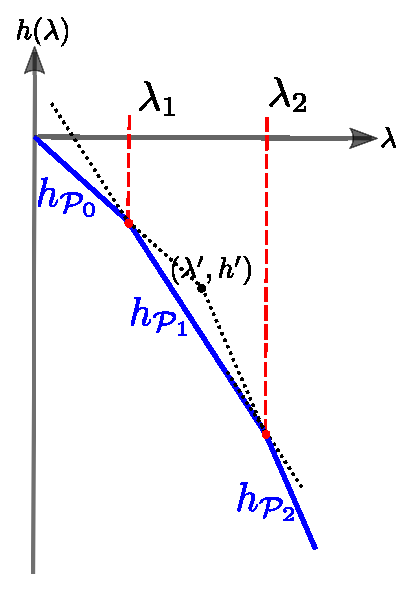
\includegraphics[width=0.4\textwidth]{psp.eps}
	\caption{piecewise linear function $h(\lambda)$ for $k=2$ where the think blue line represents $h(\lambda)$ }\label{fig:psp}
\end{figure}
Furthermore, we have $\P_0 \succeq \P_1 \dots \succeq \P_k$ \citep{narayanan}. That is, partition $\P_{i+1}$ is a refinement of $\P_i$.
And the cluster set $C_{\lambda_i} =\{C | C\in \P_i, \abs{C} > 1\}$.

A relationship between MMI and the largest threshold value is established by \citet{agg_ic} as 
\begin{equation}\label{eq:largest_threshold}
\lambda_k = \max_{B\subseteq V} I(Z_B)
\end{equation}
\subsection{Efficient Algorithm to solve PSP structure}
We call $\P_0, \dots, \P_k$ the Principal Sequence of Partition (PSP) related with $f[\P]$.
\cite{narayanan} proposes a divide and conquer approach to solve the PSP structure from equation \eqref{eq:hPLambda} for a general function $f[\P]$.
Since the optimal partition is $\P_0 = \{V\}$ when $\lambda=0$ and the partition is $\P_k=\{\{1\}, \{2\}, \dots, \{|V|\}\}$ when $\lambda$ is quite large,
his method starts from two endpoints $\lambda_i = 0, \lambda_j = +\infty$ and find the intersection of 
$h(\lambda_i)$ and $h(\lambda_j)$ at $(\lambda', h')$, which is shown in Figure \ref{fig:psp}. Then we compute a partition $\P'$ such that $h(\lambda') = h_{\P'}(\lambda')$. By definition $h(\lambda') \leq h'$ and when the strict inequality is taken we can repeat the process within $(\lambda_i, \lambda')$ and $(\lambda', \lambda_j)$ respectively. The above procedure is summarized in Algorithm \ref{alg:psp}.

\begin{algorithm}
\caption{PSP algorithm}\label{alg:psp}
\begin{algorithmic}[1]
\REQUIRE Statistics of $Z_V$ sufficient for calculating $f[B]$ for all $B \subseteq V$
\ENSURE A sorted critical value array \textbf{L} and a reverse ordered array \textbf{PSP} containing $\P_1,\dots, \P_k$.
\STATE \textbf{L}  $\leftarrow$ empty list.
\STATE $Q\leftarrow \{V\}, P \leftarrow \{ \{i \} | i \in V\}$
\STATE $\mathbf{PSP}= [Q, P]$
\STATE \texttt{Split}$(Q,P)$
\STATE sort $L$ and sort $\mathbf{PSP}$ with respect to $\succeq$ 
\FUNCTION{\texttt{Split}$(Q,P)$}
 \STATE\label{alg:gamma} $\gamma' = {1 \over \abs{P} - \abs{Q}} (f[P]-f[Q])$
 \STATE $h' = {1 \over \abs{P} - \abs{Q}}(\abs{P} f[Q] - \abs{Q} f[P])$
 \STATE $(\tilde{h}, P') = \texttt{DT}(f,\gamma')$ \footnotemark
 \IF{$\tilde{h} = h'$}
 	\STATE\label{line:11} insert $\gamma'$ to $\mathbf{L}$
 \ELSE
 	\STATE insert $P'$ to $\mathbf{PSP}$
 	\STATE \texttt{Split}$(Q, P')$
 	\STATE \texttt{Split}$(P',P)$
 \ENDIF
\ENDFUNCTION
\end{algorithmic}
\end{algorithm}
In Algorithm \ref{alg:psp}, a function \texttt{DT} (Dilworth truncation) is used to get the minimal value of Equation \eqref{eq:hPLambda}.
One implementation of \texttt{DT} is described by \cite{mac} and we omit it here.


\section{Formulation of Graph-Based Info-Clustering}\label{sec:GBIC}

In this section, we will extend info-clustering theory and focus specifically on graph model. We call our approach graph-based info-clustering (GBIC).
We will also explore various theoretical
properties of GBIC, which guides the empirical extension of GBIC to other unsupervised learning tasks.

General model of info-clustering is not very useful since we know little about the joint distribution.
We need to perform model reduction to get some useful model. 
In the following section we will use local information geometry to reduce the general model of info-clustering to our GBIC.
%. The relationship of these two special models, together with their parent model, are shown
% in the Vienn diagram in Fig. \ref{fig:relationship} % For one-column wide figures use

%\begin{figure}
%\centering
% Use the relevant command to insert your figure file.
% For example, with the graphicx package use
%  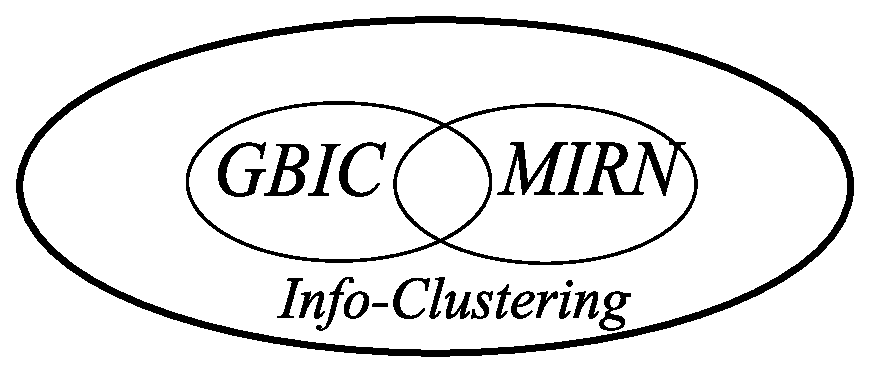
\includegraphics[width=6cm]{relationship.eps}
% figure caption is below the figuregit
%\caption{General Info clustering models reduces to GBIC or MIRN model respectively under different assumptions for the joint distribution}
%\label{fig:relationship}       % Give a unique label
%\end{figure}

%From local geometry information it is known that two random variables $X$ and $Y$ are weakly dependent if
%\begin{equation}
%P_{Y|X=x}(y) = P_Y(y) +\epsilon \phi_x(y) \sqrt{P_Y(y)}
%\end{equation}
%where $\norm{\phi_x}\leq 1$.

First we introduce the concept of weak dependency for multiple random variables.

\begin{definition}\label{def:general}
$Z_1, \dots, Z_n (n\geq 3)$ are weakly dependent if there exist a random variable $U$ such that
$(Z_1, \dots, Z_n)$ is weakly dependent with $U$ and $Z_1, \dots Z_n$ are independent conditioned
on $U$.
\end{definition}

This definition is an extension of weak dependence for two random variables mentioned in Section \ref{subsec:lig}.
For example, suppose $(Z_1, \dots, Z_n)$ are joint Gaussian and its covariance matrix concentrates on the diagonal lines.
Intuitively $Z_1, \dots, Z_n$ are near independent since the non-diagonal value of covariance matrix is very small. 
And actually we can find another $n$ dimensional Gaussian random vector $U$ such that the correlation of $Z$ and $U$ are small
and $\mathrm{Cov}(X|U)$ is diagonal matrix. Then by Definition \ref{def:general} we say $Z_1, \dots, Z_n$ are weakly dependent.
For clustering tasks, it is impossible to compute the joint distribution from limited data and it is better to make some
assumptions on the distribution. And in this article, we make the assumption of weak dependency, which is indeed better than totally
independence and competitive to parametric Bayesian assumption.

Let $\P$ be the partition of $V=\{1,2,\dots, n\}$. We claim:
\begin{theorem}\label{thm:DPX}
If $Z_1, \dots, Z_n$ are weakly dependent, then
\begin{equation}\label{eq:PXV}
D(P_{Z_V} || \prod_{C\in \P} P_{Z_{C}}) = {1 \over 2}\sum_{\substack{(i,j) \not\in C\\ C\in \P}} \norm{B_{ij}}_F^2 + o(\epsilon^2)
\end{equation}
where $B_{ij}$ is the $B$ matrix between random variable $Z_i$ and $Z_j$.
\end{theorem}
We can see that Theorem \ref{thm:DPX} is an extension of the approximation of mutual equation in Equation \eqref{eq:Ixy} to the case of multiple random variables.

% To get the required KL-Divergence under a given partition, we only need to make a
%summation of these weight terms.

Theorem \ref{thm:DPX} is a statement about random variables. Now we expand it to data samples. Given a $K-$cluster dataset with $n$ samples, each cluster is regarded as a random variable. 
Assuming the $i$-th cluster $Z_i$ with alphabet size $\abs{\mathcal{Z}_i}$, totally
we have $\sum_{i=1}^K \abs{\mathcal{Z}_i} = n$.
Since $Z_i$ and $Z_j$ are weakly independent for $i\neq j$, we have
\begin{equation}\label{eq:phi_w}
P_{Z_i Z_j}(z_i, z_j) = P_{Z_i}(z_i)P_{Z_j}(z_j) + \epsilon \sqrt{P_{Z_i}(z_i)P_{Z_j}(z_j)} \phi_{Z_i Z_j}(z_i, z_j) + o(\epsilon)
\end{equation}
Therefore from Equation \eqref{eq:Ixy}, $\norm{B_{ij}}_F^2 = \epsilon^2 \sum_{z_r \in \mathcal{Z}_i, z_s \in \mathcal{Z}_j} \phi^2_{Z_i Z_j}(z_r, z_s)$ and Equation \eqref{eq:PXV} can be expanded as
\begin{equation}\label{eq:PXV_Data}
D(P_{Z_V} || \prod_{C\in \P} P_{Z_{C}}) =
{\epsilon^2\over 2}\sum_{\substack{(i,j) \not\in C\\ C\in \P}}
\sum_{z_r \in \mathcal{Z}_i, z_s \in \mathcal{Z}_j}  \phi^2_{Z_i Z_j}(z_r, z_s) + o(\epsilon^2)
\end{equation}
We can treat the term
$\phi^2_{Z_i Z_j}(z_r, z_s)$ as the weight of an edge for a graph with $n$ nodes.
Each vertex of the graph is corresponding to a data sample.
To simplify the notation, let $w_{rs} = \phi^2_{Z_{d(z_r)}Z_{d(z_s)}}(z_r, z_s)$ \footnote{When $d(z_r) = d(z_s)$, we can still formally define $w_{rs}$ to be some value larger than $\phi^2_{Z_i Z_j}(z_r, z_s)$ for $i\neq j$.} where $d(z_r)$ maps the vertex to its underlining random variable index, $1\leq r,s \leq \abs{V}$.
We can also expand each $Z_i$ to its alphabet and treat $\P$ as the partition of graph vertices.
Suppose the graph $G(V, E)$ we considered is directed
\footnote{Without loss of generality we only consider directly graph in this article to reduce computational cost in algorithm part},
we can define the graph in-cut function $f(C)$ for $C\subseteq V$ as $f(C) = \sum_{i\not\in C, j\in C, (i,j) \in E} w_{ij}$, which is the total weight of edges coming
into $C$.
From Equation \eqref{eq:PXV_Data}, we can characterize the KL divergence by the total inter-cluster edge weight as
\begin{equation}\label{eq:PXV_Data_Simplified}
D(P_{Z_V} || \prod_{C\in \P} P_{Z_{C}}) = \epsilon^2 \sum_{C \in \P} f(C)+ o(\epsilon^2)
\end{equation}
Notice that for directed graph, each edge weight is counted only once in the summation. Therefore there is no need to divide 2 in
Equation \eqref{eq:PXV_Data_Simplified}.
Combining Equation \eqref{eq:IZV} and \eqref{eq:PXV_Data_Simplified} we get the expression for the second order coefficient of multivariate mutual information (MMI):
\begin{definition}[MMI of GBIC]\label{def:ms}
	\begin{align}
	I_{\P}(Z_V) & := \frac{ f[\P] }{  \abs{\mathcal{P}} - 1 } \textrm{ where } f[\P] = \sum_{C\in \P}f(C) \label{eq:ms_first}\\
	I(Z_V) & := \min_{\mathcal{P} \in \Pi'(V)} I_{\mathcal{P}}(Z_V)  \label{eq:ms}
	\end{align}
\end{definition}

With a little abuse of terminology and notation, we use $I_{\P}(Z_V)$ to represent the second order coefficient of MMI and call it the MMI of graph-based mutual clustering (GBIC). 


We can also compute MMI of GBIC for subgraph $G'(V',E')$ of $G$, denoted by $I(Z_{V'})$. When $V'=\{i,j\}$, we have $I(Z_{V'})=w_{ij}$ from the above definition.

To reduce the general model of info-clustering to GBIC, we not only use the weak dependency assumption, but also assume that each random variable $Z_i$ only takes discrete values from the observed samples $\mathcal{Z}_i$. The second assumption is also plausible, since it can be seen as an non-parametric approach restricted to discrete distribution. When the number of observed samples is large, it is approximating a continuous distribution.

To apply GBIC on empirical experiment, $w_{ij}$ should be chosen properly. $w_{ij}$ measures the relevance of events $Z_{d(z_i)} = z_i$
and $Z_{d(z_j)} = z_j$. 
From its definition \eqref{eq:phi_w}, $w_{ij} \geq 0$. When $w_{ij} = 0$, the two events are independent and we say there is no edge between
node $i$ and node $j$. The larger $w_{ij}$ takes, the more relevant the two events are. The relevance can be regarded as similarity of data samples 
from engineering prospective. The choice of $w_{ij}$ is not unique. The rbf kernel $w_{ij} = \exp(-\gamma \norm{z_i - z_j}^2)$ is a common choice
where $\gamma$ is a positive parameter to be tuned.

To perform clustering tasks based on our GBIC model, we follow the same procedure as the general info-clustering model. That is, we proceed in a divisive way as Equation \eqref{eq:CZV}. Finally, we can get the cluster tree $\mathcal{T}$.

Based on our assumption, the tree leaf nodes are data samples and they are joined together at a stem node $\mathcal{Z}_i$. It is also possible that $\abs{\mathcal{Z}_i} = 1$. In such case, we say $Z_i$ is an outlier.


\begin{example}
\begin{figure}
	\centering
	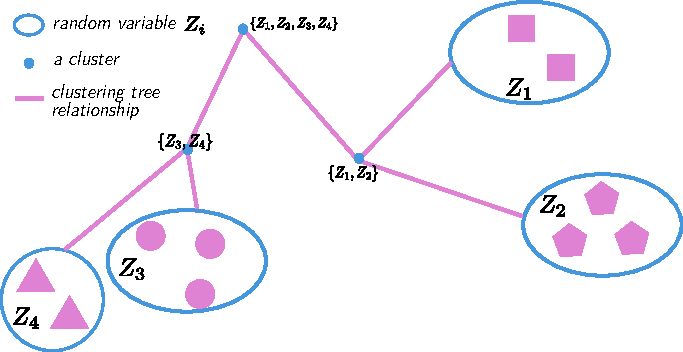
\includegraphics[width=\textwidth]{GBIC.pdf}
	\caption{hierarchical clustering tree based on GBIC. There are 10 data samples and 4 underlining clusters. The cluster of triangles joins the cluster of circles while the cluster of squares joins the cluster of pentagons. Finally, the intermediate two super-clusters joins at the tree root.}\label{fig:ta}
\end{figure}
Consider 10 data samples and their feature vectors are on Euclidean plane, as shown in Figure \ref{fig:ta}. The underlining graph with 10 nodes is weighted  by $w_{ij} = \exp(-\norm{z_i - z_j}^2)$. Let $Z_1, Z_2, Z_3, Z_4$ represents the square, pentagon, circle and triangle samples respectively. We can write the clustering solution \footnote{computed by Algorithm \ref{alg:psp} introduced in the next Section} as:
\begin{equation*}
\P = 
\begin{cases}
\{\{Z_1,Z_2,Z_3,Z_4\}\} & \lambda < 0.2 \\
\{\{Z_1,Z_2\},\{Z_3,Z_4\}\} & 0.2 \leq \lambda < 0.22 \\
\{\{Z_1\},\{Z_2\},\{Z_3,Z_4\}\} & 0.22 \leq \lambda < 0.59\\
\{\{Z_1\},\{Z_2\},\{Z_3\},\{Z_4\}\} & 0.59 \leq \lambda \geq 0.98
\end{cases}
\end{equation*}
When $\lambda > 0.98$, some clusters are split further to data samples.
Although the clustering tree itself does not distinguish
$\{\{Z_1\},\{Z_2\},\{Z_3,Z_4\}\}$ from $\{\{Z_1,Z_2\},\linebreak[2] \{Z_3\}, \{Z_4\}\}$,
by threshold value constraints the partition $\{\{Z_1,Z_2\} \linebreak[2] ,\{Z_3\}, \{Z_4\}\}$ does not exist.
\end{example}

Since GBIC is a special model of info-clustering, all theoretical properties of info-clustering apply to GBIC as well. Besides, we will give some extra properties (Proposition \ref{prop:triangle} to \ref{prop:main}), which are specific to GBIC model.

We notice that the weight given in Equation \ref{eq:ms_first} is additive. This tends to produce trivial hierarchical structure when the scheme of weights is not chosen properly.
For example, it happens if all weights value are within the range of $[a, 2a]$ where $a>0$. This is due to the following proposition:

\begin{proposition}\label{prop:triangle}
Let $w_{ij}=0$ if $(i,j)\not\in E$. If $w_{ij} + w_{jk} \geq w_{ki}$ for any different triple $i, j, k \in V$, then the info-clustering solution is trivial\footnotemark.
\end{proposition}
\footnotetext{By trivial solution we mean only $\{V\}$ is a cluster, or the hierarchical tree contains only root and leaves.}

Using Proposition \ref{prop:triangle}, a special case is a complete graph $G(V,E)$ with equal weight $r$ on each edge. We then have $I(Z_{V})=\frac{nr}{2}$ where $n=\abs{V}$. The clustering result is trivial for such graph. However, if we add some edges between such two complete graphs, an interesting problem is to investigate when GBIC can recover the two node sets of the complete graph. A subset is recoverable if this set is a cluster in GBIC model.
For this problem, we have the following proposition:

\begin{proposition}\label{prop:reweight}
Suppose $S_1, S_2 $ are complete graph node set with $\abs{S_1}=\abs{S_2}=n$ and equal weight $w_{ij}=r$. There are $m$ edges between the two graphs and all inter-connection edges have equal weight 1. The vertex set for the whole graph is $V=S_1\cup S_2$. If $m <\frac{nr}{2}$  we have
$I(Z_V) = 
m$ and the recovery is possible. If $m\geq \frac{nr}{2}$, the recovery is not possible.
\end{proposition}

In later part we will show how the result of Proposition \ref{prop:reweight} can be used to build a hierarchical discovery method in community detection problems.

Besides considering static graph $G$, there is often a problem to consider which cluster a new observation belongs to.
To model this, we add a new node $i'$ to the existing graph $G$. Let $\gamma_N$ represents the largest critical value.
From Equation \eqref{eq:largest_threshold}, assume $\gamma_N = I(Z_B)$ and $V'=B \cup \{i'\}$. We can compute $\gamma'_N$ for the new graph $G(V', E(V'))$ and compare it with $\gamma_N$. $\gamma'_N \geq \gamma_N$ holds in general. It can be shown that we do not need to compute $\gamma'_N$ to determine whether $\gamma'_N>\gamma_N$. We summarize our main result as follows:
\begin{proposition}\label{prop:main}
\begin{equation}
\gamma'_N > \gamma_N \iff  \sum_{i \in B} w_{ii'} > \gamma_N 
\end{equation}
\end{proposition}
Proposition \ref{prop:main} gives a method to check whether the newly added node destroys the outermost clustering structure of the hierarchical tree.  For example, suppose we add a triangle sample to Fig \ref{fig:ta} from the bottom left position. If it is near to the triangle cluster, the newly added sample is belonging to the cluster. Otherwise it is an outlier. In later part we will show more precisely how this result can be used to deal with outlier detection problem.

\section{Improved PSP Algorithms}\label{sec:alg}
To compute the clusters in GBIC, we first compute the PSP structure defined in Equation \eqref{eq:PSP_structure}. Then from the established equivalence of the nested partition and the clustering tree, the hierarchical
clustering results are obtained. This procedure is the same with the general model of info-clustering and the algorithm to computing PSP structures is not limited to GBIC. In this section, we will give a faster algorithm to compute PSP structures for a general directed graph.

\subsection{Formulation of PSPI}
Our improved algorithm will use the same \texttt{DT} routine as mentioned Algorithm \ref{alg:psp}. We notice that different invocation of \texttt{DT} is independent and does not utilize the intrinsic hierarchical structure in Algorithm \ref{alg:psp}. If the hierarchical tree structure is used, we can invoke \texttt{DT} on smaller graph in later computation and make the total computation one order of magnitude faster than previous.

To be more specific, suppose we get $P_i = \{C_1, \dots, C_t\}$ for the first invocation of DT. Then we can compute PSP for each $C_i(i=1,\dots, t)$ respectively and construct those $P_j(j>i)$ from the subgraph computation. For $P_j(j<i)$, we can contract the graph $G$  to $G^t$ which has $t$ nodes by contracting each $C_i$ to a single node. By applying DT to $G^t$ can we get $P_j(j<i)$. We summarize our improved version (PSPI) in Algorithm \ref{alg:psp_i_simplified} and illustrate the algorithm by Figure \ref{fig:pspi}.

\begin{algorithm}
	\caption{An Improved Principal Sequence of Partition Algorithm}\label{alg:psp_i_simplified}
	\begin{algorithmic}[1]
		\REQUIRE a directed graph $G(V, E)$; edge weight map $c(e)$ for $e\in E$
		\ENSURE a hierarchical tree $\mathcal{T}(K, E)$ where $K \subseteq 2^{V}$ is node set and $E$ is edge set
		\STATE initialize tree $\mathcal{T}$ with $V$ as root node, $\{j\}(j \in V)$ as leaf node and no stem node
		\STATE \texttt{Split}($G, V$)
		\FUNCTION{\texttt{Split}($\widetilde{G}, \widetilde{V}$)}
		\STATE $w$ is the summation of all edge weights of $\widetilde{G}$ 
		\STATE $\gamma' = \frac{w}{\abs{V(\widetilde{G})}-1}$ where $V(\widetilde{G})$ is the node set of graph $\widetilde{G}$ \label{alg:gamma_apostrophe}
		\STATE $(\tilde{h}, P') = \texttt{DT}(\widetilde{G}, \gamma')$ where $\P'$ is the minimizer of $h(\gamma')$ in equation \eqref{eq:hPLambda} and $\tilde{h}$ is the corresponding minimal value  \label{line:DT}
		\IF{$\tilde{h} = - \gamma'$}
		\STATE add edge weight $\gamma'$ in $\mathcal{T}$ starting from $\widetilde{V}$ to its children
		\ELSE
		\FOR{$S$ in $P'$ and $\abs{S}>1$}
		\STATE make each children of $\widetilde{V}$ in $\mathcal{T}$ have new parent $S$		
		\STATE make the parent of $S$ be $\widetilde{V}$
		\STATE \texttt{Split}($\widetilde{G}[S], S$) where $\widetilde{G}[S]$ is the subgraph of $\widetilde{G}$ restricted on $S$ \label{line:SplitDown}
		\STATE contract $S$ to a single node in $\widetilde{G}$ % graph \widetilde{G} is modified
		\ENDFOR 
		\STATE \texttt{Split}($\widetilde{G}, \widetilde{V}$)		\label{line:SplitUp}
		\ENDIF
		\ENDFUNCTION
	\end{algorithmic}
\end{algorithm}

\begin{figure}
\centering
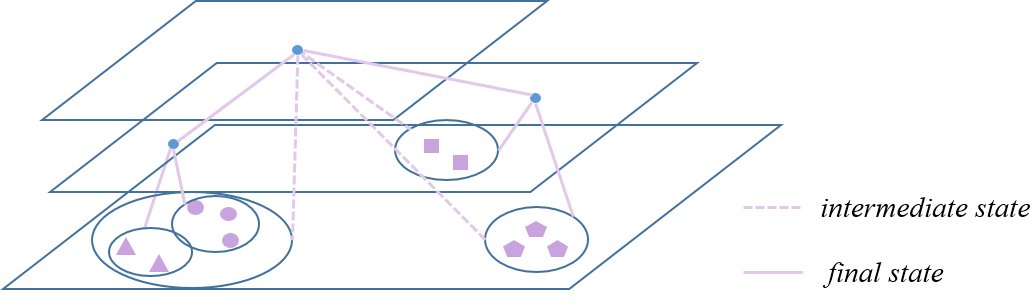
\includegraphics[width=0.9\textwidth]{improved_alg.png}
\caption{Illustration of PSPI: The intermediate state is achieved first by Line \ref{line:DT} in Algorithm \ref{alg:psp_i_simplified};
Then the tree ellipses are divided further in Line \ref{line:SplitDown} and are also clustered upwards to formal the final state in Line \ref{line:SplitUp}.}\label{fig:pspi}
\end{figure}

We analyze the time complexity of Algorithm \ref{alg:psp_i_simplified} for dense graphs. That is, we suppose $\abs{V} = n, \abs{E} = O(n^2)$. For sparse graphs the bound can be improved. We use a conclusion that \texttt{DT} routine has $O(n^4)$ time complexity and the time complexity for Algorithm \ref{alg:psp} is $O(n^5)$ \citep{pin}.

We use $T(n)$ to represent the time complexity of \texttt{Split} when the graph has $n$ nodes.
From Algorithm \ref{alg:psp_i_simplified}, the recursive relationship for $T(n)$ is
\begin{equation}\label{eq:Tn}
T(n) = \max \{ C n^4 + \sum_{i=1}^k T(n_i) + T(k)\delta_{k<n} | \sum_{i=1}^k n_i = n, n_i \in \mathbb{Z}_{+} \}
\end{equation}	
In \eqref{eq:Tn}, $Cn^4$ is the time complexity of \texttt{DT}. $\delta_{k<n} = 1$ when $k<n$, otherwise $\delta_{k<n}=0$. We have the following proposition:
\begin{proposition}\label{prop:alg_complexity}
	 If $n_i \leq \frac{n}{2}, \textrm{ for } i=1,\dots,k$ and $ k \leq \frac{n}{2}$  hold in equation \eqref{eq:Tn}, then $T(n) = O(n^4)$.
\end{proposition}

The condition in Proposition \ref{prop:alg_complexity} restricts the shape of the clustering tree. For each non-leaf node, its children and the number of samples in each children are limited. However, the limitation is not so strict and
many near-balanced trees satisfied the condition. Therefore, we can say that under this mild condition of Proposition \ref{prop:alg_complexity},
our PSPI has time complexity $O(n^4)$, which is one order of magnitude faster than $O(n^5)$ of Algorithm \ref{alg:psp}.

If the worst case scenario is considered, that is, the depth of the hierarchical tree is of order $O(n)$. Then it is inevitable to invoke \texttt{DT} $O(n)$ times.
In this scenario, the complexity bound for $T(n)$ is $C(3^4+4^4 + \dots + n^4) \sim \frac{1}{5}Cn^5$, which is $5$ times faster than $Cn^5$ of Algorithm \ref{alg:psp}.

\subsection{Empirical Comparison of Different PSP Algorithms}
Another improvement to compute PSP is formulated by \cite{kolmogorov} using parametric maximum flow.
This improvement can also achieve $O(n^4)$ time complexity theoretically. 
In this section, we compare our PSPI with Algorithm \ref{alg:psp} and Kolmogorov's algorithm
using two datasets with different edge density.

The first dataset is four Gaussian blobs with equal size and we can vary the number of points in each blob. The dataset with 100 points in total is the same with that used in 
Section \ref{subsec:dc}. The second dataset is a two-level graph with $s^3$ nodes. The dataset with $s=4$ is the same with that used in Section \ref{subsec:cd}.
We can construct a graph from the first dataset and the edge weight is computed with the rbf kernel. The characteristics of these two datasets are summarized in
Table \ref{tab:alg_compare}.
\begin{table}[!ht]
\centering
\begin{tabular}{ccc}
\hline
name & weight type & density \\
\hline
Gaussian-blobs & int & $|E|=O(|V|^2)$\\
Two-level graph & float & $|E|=O(|V|^{3/2})$\\
\hline
\end{tabular}
\caption{Dataset properties used in algorithm speed comparison} \label{tab:alg_compare}
\end{table}
We use CPU times to measure the time complexity of the algorithms. By varying the number of nodes, we can get the experiment results, shown in Figure \ref{fig:esc}.
As can be seen, our implementation is much faster than previous ones.

\begin{figure}
	\centering
	\begin{subfigure}{0.45\textwidth}
		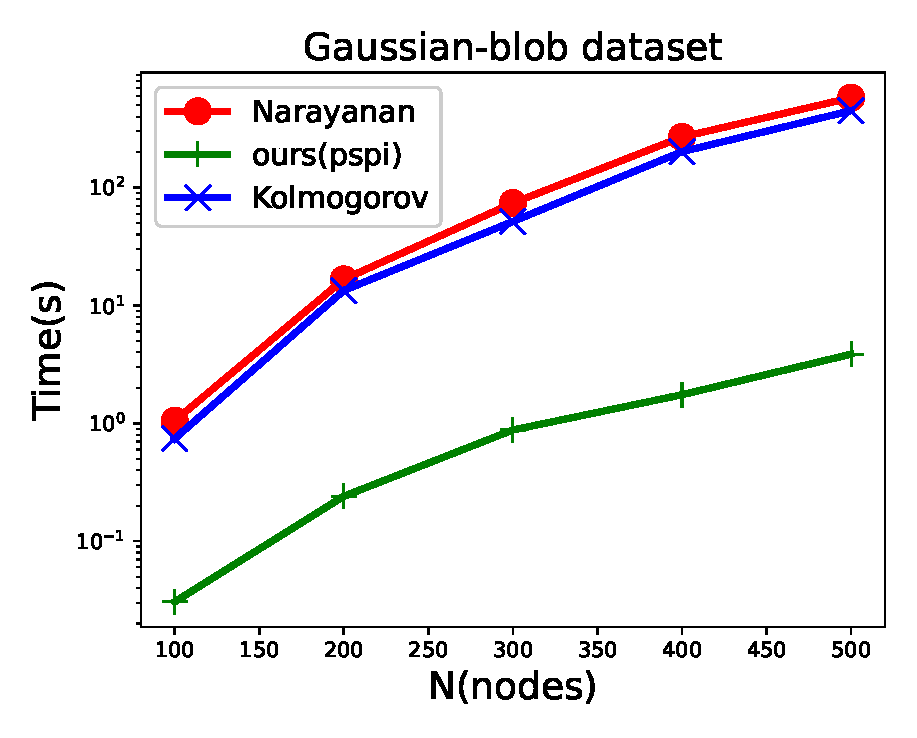
\includegraphics[width=\textwidth]{pic/2019-08-26-gaussian.eps}
	\end{subfigure}
	\begin{subfigure}{0.45\textwidth}
		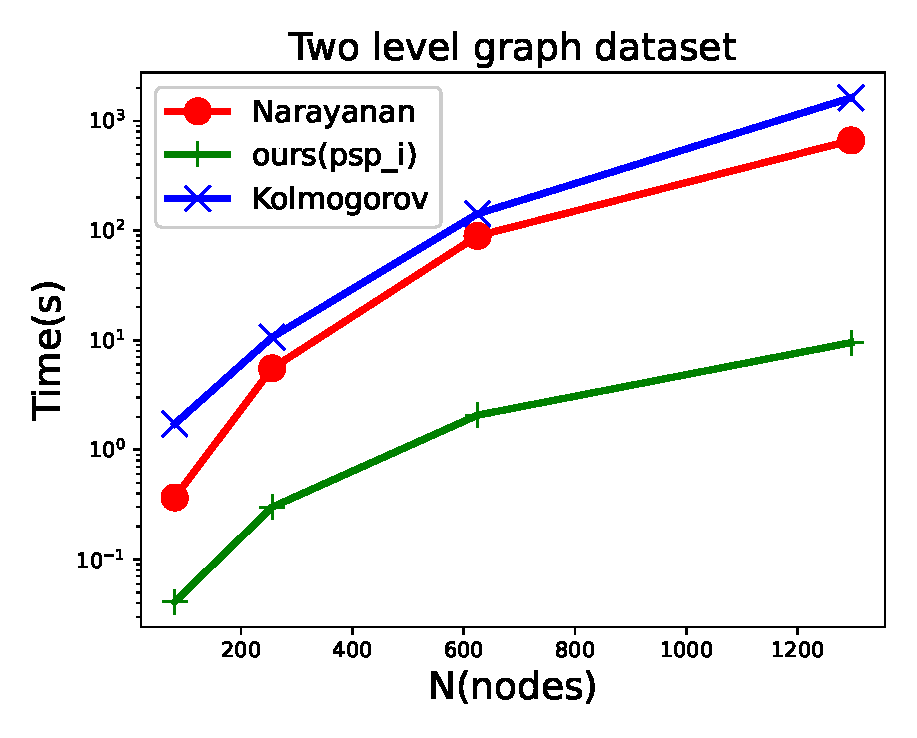
\includegraphics[width=\textwidth]{pic/2019-09-19-two_level.eps}
	\end{subfigure}
	\caption{Empirical speed comparison of different PSP algorithms}\label{fig:esc}
\end{figure}

We notice that parametric flow based PSP \citep{kolmogorov}  does not perform well in practice. This may be related with the extra cost to construct intermediate graph structures and maintain concurrent threads, whose time overhead can not be neglectable in implementation.

\section{Empirical Study of GBIC}\label{sec:es}
In this section, we apply GBIC to various unsupervised learning problems including clustering analysis, community detection, link prediction and outlier detection.
In some problems we need to extend GBIC and give the corresponding decision criterion based on the clustering tree of GBIC.
These decision criteria are empirically inspired and performs well in our experiment. Our experiments
include synthetic and real-world dataset and we will compare GBIC with classical methods and Bayesian inference.

\subsection{Clutering Analysis Scenario}\label{subsec:dc}
For clustering analysis task, we are given $n$ data, each with a feature vector of length $m$.
To use GBIC on such scenario, we need to construct a similarity matrix from the feature vectors. Each element of the similarity matrix corresponds a weight value of the underlining graph. Some classical clustering methods like Spectral Clustering also follow the similarity matrix approach. Practical study shows that rbf kernel and Laplacian kernel are good choice to construct the matrix.
For these type of similarity, the graph is quite dense and to reduce the computational cost we can treat very small weights as zero. That is, we set a threshold for the weights to remove some edges in the graph. We can also use k-nearest neighbors to generate discrete similarities. It is hard to say which similarity metric is better than others and it depends on specific problems. Besides, the hyper-parameters of the metric can be tuned as well.

After we get the clustering tree, we can get a proper flat clustering by extracting one partition from the tree. This is typical for most hierarchical clustering method. Then we can compare different clustering method, whether they are hierarchical or not. We use 3 different datasets for such purpose.

\begin{enumerate}
\item Four Gaussian blobs with unit variance and centers at $(3,3), (3,-3), (-3,3),  \linebreak[4](-3,-3)$ respectively.  We generate 25 points for each blob.
\item Three concentric circles with radius $0.1,0.2,0.3$ and number of data points as $60, 100, 140$. The angles of these points are uniform distributed and they also oscillate along the radius direction.
\item UCI glass dataset with 214 samples, 6 classes, 9 dimensions of feature.
\end{enumerate}
We use adjusted rand index as the metric to score different clustering method.
The best performance for each algorithm is shown in Table \ref{tb:e1}.
It can be seen from the table that GBIC is better than other clustering algorithms.
\begin{table}[!ht]
\centering
\InputIfFileExists{compare_3.tex}{}{}
\caption{ accuracy for different clustering algorithms }\label{tb:e1}
\end{table}

To compare different hierarchical clustering method, it is better to compare the clustering tree directly.
For this purpose,
we use the gene-expression dataset from \cite{khan2001classification}.
Because we do not know the ground truth, we can split the features and apply the clustering algorithms on two dataset with partial features respectively and compare the resulting clustering tree. By doing so we can also test the stability of each clustering method.

We compare GBIC with agglomerative hierarchical clustering (average distance) and Bayesian Rose tree \citep{blundell2011discovering}. The tree similarity metric is Robinson-Foulds distance, which is the number of steps to transform one tree to another (A step is either adding or removing an edge) \citep{day1985optimal}. We vary the samples of data and the results are shown in Figure \ref{fig:shc}. As can be seen, for the classical hierarhical method the trees tend to have more edges and the distance is large. The distance of GBIC and that of Bayesian Rose tree are near when $n$ is large. But when $n$ is small, our method performs best.

\begin{figure}
\centering
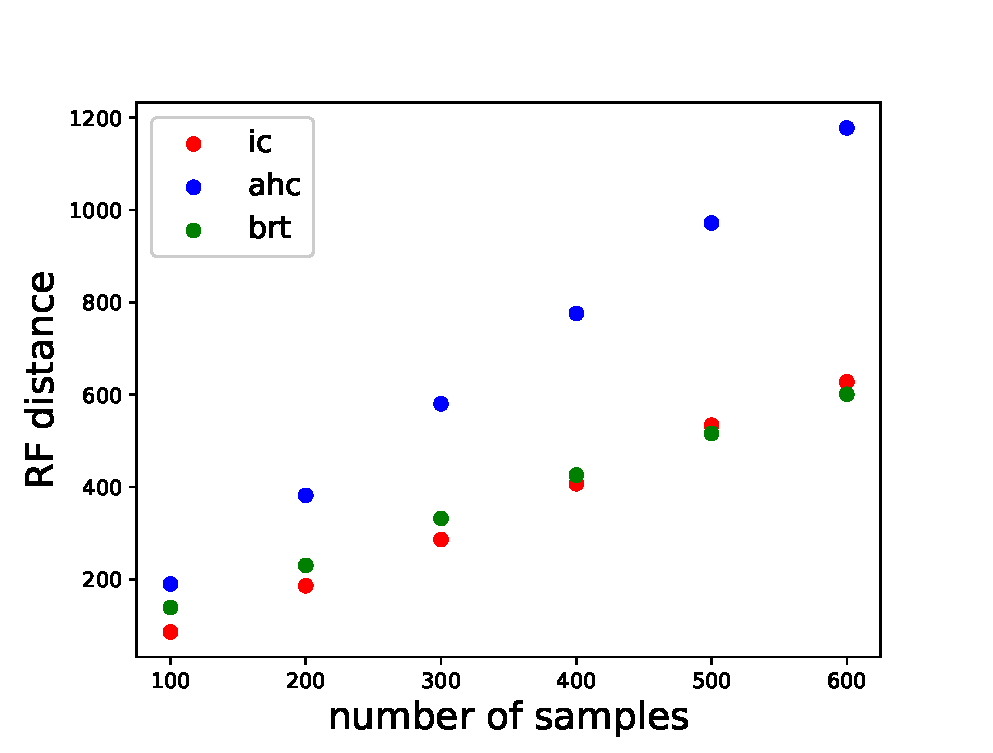
\includegraphics[width=6cm]{pic/plot_results.eps}
\caption{Comparison of the stability of hierarchical clustering method}\label{fig:shc}
\end{figure}

\subsection{Community Detection}\label{subsec:cd}
Community Detection problems can be regarded as finding a proper partition of a given graph and we call each subgraph in the partition a community. There are many good algorithms
to find the flat partition which splits the graph into several non-overlapping subgraphs \citep{malliaros2013clustering}. However, it is a hard problem to make inference on the hierarchical structure of a complex graph automatically.
In this subsection we use experiments to demonstrate that GBIC
can achieve success to recover the hierarchical structure of a two-level graph upon properly defined ``edge weight''.

To apply GBIC on community detection problems, we can not treat each edge with equal weight otherwise it is very possible to obtain only trivial clustering results due to Proposition \ref{prop:triangle}. Inspired by Proposition \ref{prop:reweight}, we use the following weighting scheme:

\begin{equation}\label{eq:wij_scheme}
    w_{ij} = 1 + \abs{\{k | (i,k),(j,k) \in E \}} \textrm{ for } (i,j) \in E
\end{equation}
This weight assignment scheme for $w_{ij}$ is the number of one and two hop paths between $i$ and $j$. For edges in a complete graph, it is equivalent to take $r=n$ in the model problem of Proposition \ref{prop:triangle}. Then approximately it needs
at least $\frac{n^2}{2}$ edges to make the two subgraphs unrecoverable.
Beyond the theoretical analysis of two community model, now we consider a more complex structure and empirically justify the weighting scheme of Equation 
\eqref{eq:wij_scheme}.

\begin{figure}
	\centering
	\begin{subfigure}{0.45\textwidth}
		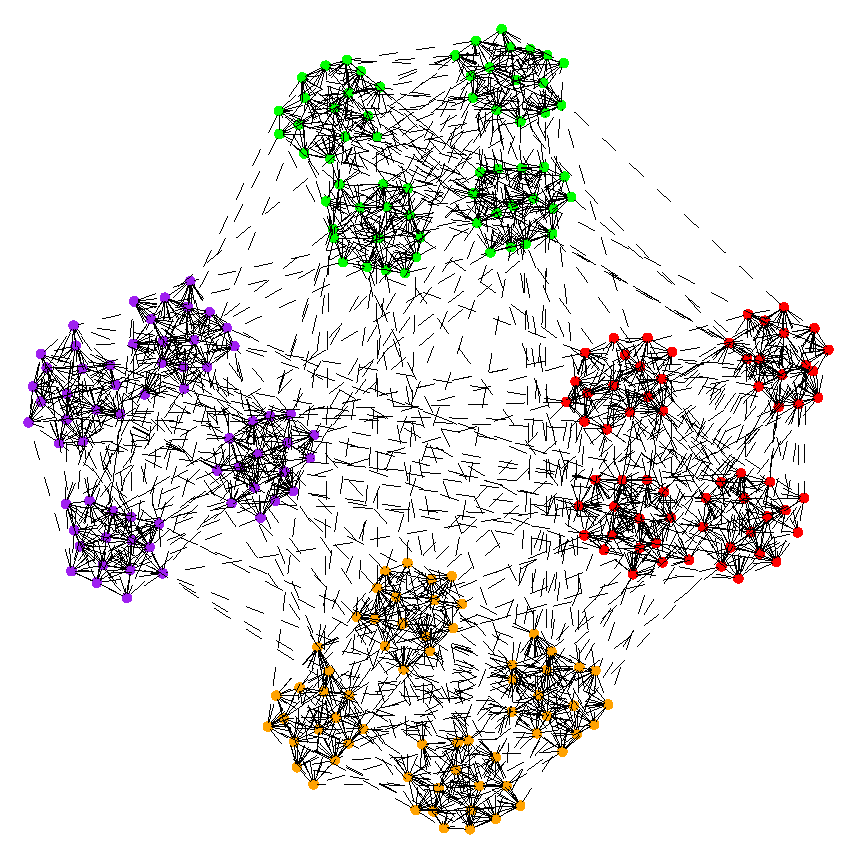
\includegraphics[width=\textwidth]{pic/two_level.eps}
		\caption{a community with two hierarchical levels with $z_{\mathrm{in}_1} = 14,$ $z_{\mathrm{in}_2} = 3, z_{\mathrm{out}}=1$.}\label{fig:c1}
	\end{subfigure}
	\begin{subfigure}{0.45\textwidth}
		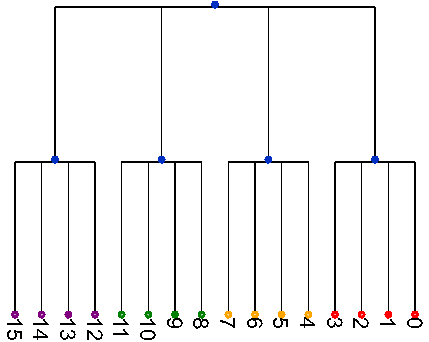
\includegraphics[width=\textwidth]{pic/tree_info-clustering.pdf}
		\caption{hierarchical tree obtained by graph-based info-clustering for left figure. The tree leaves with the same ancestor are merged for clarity.}\label{fig:c2}
	\end{subfigure}
	\caption{Community Detection Experiment Illustration}
\end{figure}
We use a two-level artificial dataset proposed in \cite{RN22}. 
The community structure is shown in Fig. \ref{fig:c1}. It has 4 communities in macro-level, and each macro community contains 4 micro communities. We use $z_{\mathrm{in}_1}$ to represent the internal average degree of nodes within micro community; $z_{\mathrm{in}_2}$ as node degree between different micro communities but within one macro community; $z_{\mathrm{out}}$ as node degree between different macro communities. By varying one and fixing the other two in $\{z_{\mathrm{in}_1}, z_{\mathrm{in}_2}, z_{\mathrm{out}} \}$ we get different sets of experiment.
To compare the deduced hierarchical tree structure with the ground truth, we use the normalized Robinson-Foulds distance as the metric, which lies within $[0,1]$. We compare the RF distance of GBIC with that of GN (Girvan-Newman algorithm) and BHCD (a kind of Bayesian Hierarchical method for graph structure by \cite{RN23}). The result is shown in Fig. \ref{fig:cdr}. As can be seen from Fig.\ref{fig:cdr}, in either case, graph-based info-clustering can produce more similar tree structures than other methods.
\begin{figure}
	\centering
	\begin{subfigure}{0.33\textwidth}
		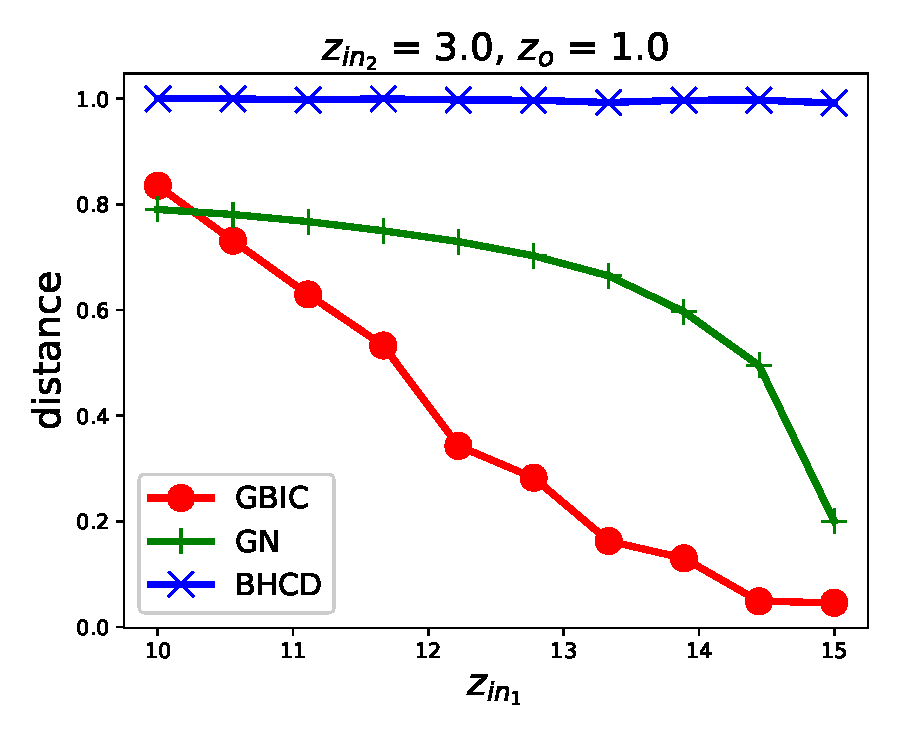
\includegraphics[width=\textwidth]{pic/z_in_1.eps}
		\caption{}
	\end{subfigure}~
	\begin{subfigure}{0.33\textwidth}
		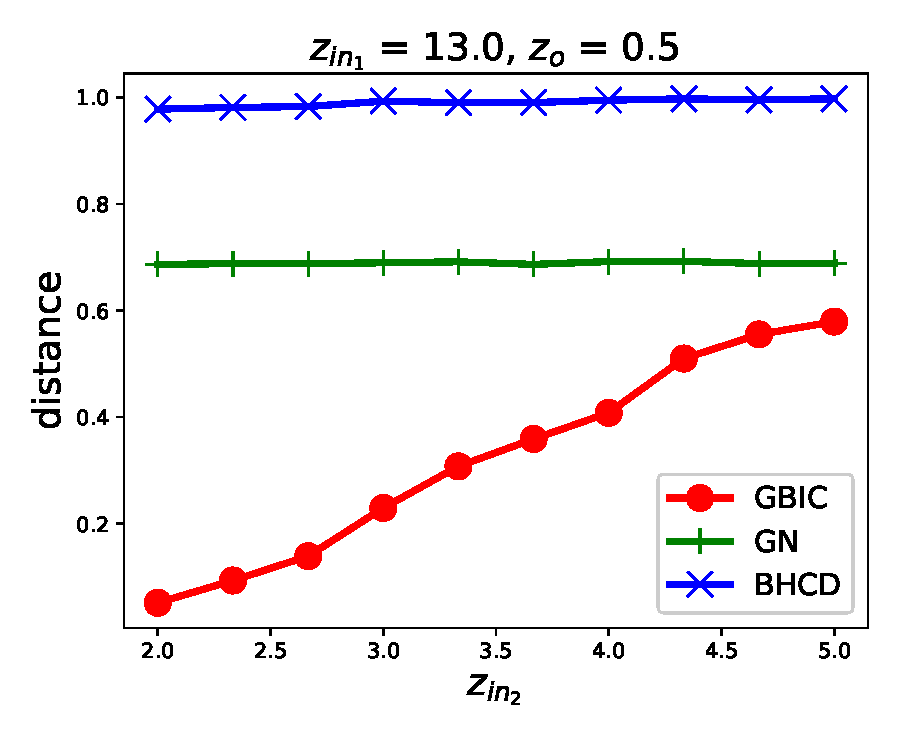
\includegraphics[width=\textwidth]{pic/z_in_2.eps}
		\caption{}
	\end{subfigure}~
	\begin{subfigure}{0.33\textwidth}
		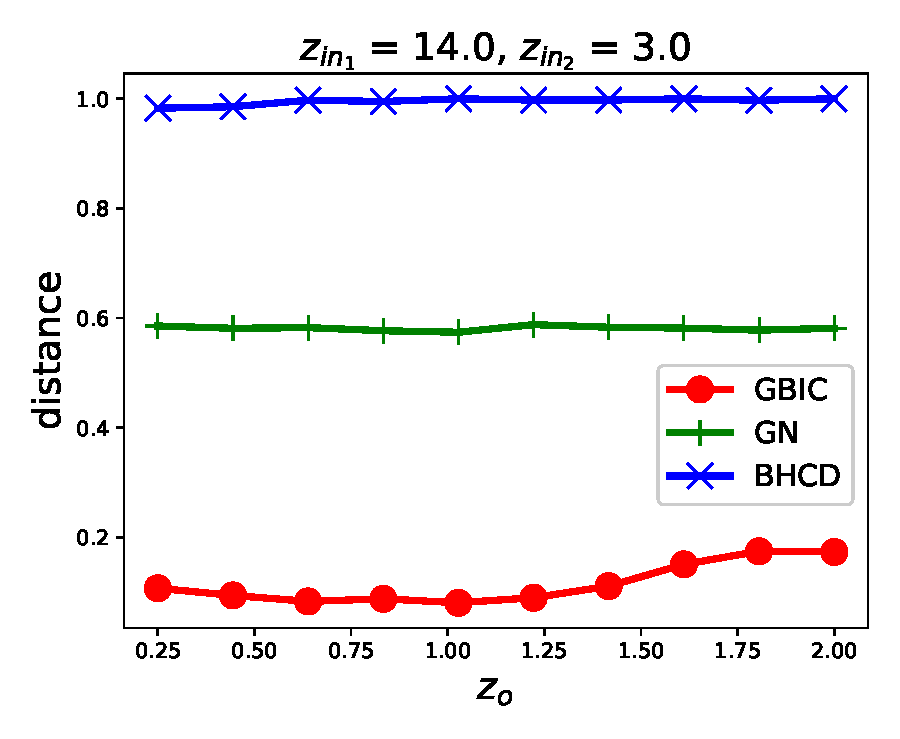
\includegraphics[width=\textwidth]{pic/z_o.eps}
		\caption{}
	\end{subfigure}
	\caption{Distance comparison between different hierarchical community detection method. Smaller distance indicates more similar structure with the ground truth tree.}\label{fig:cdr}	
\end{figure}
\subsection{Link Prediction}
Link Prediction problem is predicting whether an unobserved edge exists between two nodes in a graph \citep{liben2007link}.  GBIC does not give an explicit way to make prediction. Here we give a heuristic prediction scheme based on the hierarchical tree $T$ generated by GBIC.
Our problem is that given node $(i,j) \not\in E$, we should make a prediction whether they have an connected edge.
Let $A[i]$ denote the set of all ancestors of leaf node $i$ in the clustering tree. Without loss of generality we suppose $\abs{A[i]} \leq \abs{A[j]}$.
We split the scenario 
into two cases:
\begin{enumerate}
\item If node $A[i] \subseteq A[j]$, we test whether the addition of the edge with weight $w$ will split them. To be more specific, we consider the subgraph consisting of all the sibling of $i,j$. We add edge $(i,j)$ and do GBIC on this sub-graph. If the partition is trivial, then we conclude that the connected edge exists. Otherwise, the edge does not exist.

\item If node $A[i] \not\subseteq A[j]$, we test whether the addition of the edge will join them. The test is bidirectional. Suppose $I$ is the parent node of $i$ and it consists of several parts. We add edge $(i,j)$ and consider the subgraph $I \cup \{j\}$. If the largest critical value becomes larger than before, then there is an edge bewteen $i,j$. Otherwise, consider the other part of the test for $J$ including $j$. If neither of the two tests succeed, we conclude that there is no edge between $i,j$. To test whether the largest critical value becomes larger than before, we will use Proposition \ref{prop:main},  thus avoiding complicated solution of GBIC for subgraphs.
\end{enumerate}

Co-authorship datasets are a typical exemplar to compare different link prediction methods. We use the NIPS-authorship dataset as done by \cite{RN23}.
Since the graph is sparse and it is hard to predict for some node with little connection information, we restrict the network to the 234 nodes whose degrees are largest. Since the prediction  is a hypothesis testing problem, we use true positive rate (TPR), true negative rate (TNR) and accuracy (ACC) as the evaluation metric. We compare GBIC with BHCD and a local prediction method based on a metric called Resource Allocation Index \citep{zhou2009predicting} and the result is shown in Table \ref{tab:nips}. It can be seen that for TPR our method achieves higher score
and for other metrics our method is near the best.
\begin{table}
\centering
\begin{tabular}{cccc}
\hline
     Method      &   TPR    &   TNR    &   ACC    \\
\hline
 info-clustering & 80.068\% & 99.472\% & 99.365\% \\
      bhcd       & 73.514\% & 99.590\% & 99.446\% \\
\hline
\end{tabular}
\caption{Comparison of different link prediction methods on Authorship dataset}\label{tab:nips}
\end{table}



\subsection{Outlier Detection}\label{subsec:od}
Outlier Detection is the identification of abnormal data (called outliers) which differs from the majority of the data (called inliers) \citep{grubbs1969procedures}.
To apply our GBIC method to this problem, we consider the case when we are required to detect outliers in a multi-class dataset and we are required to
extract a partition $\{C_1, \dots, C_K, \{x_1\}, \dots, \{x_M\}\}$ from the PSP where $K$ is the number of clusters and $M$ is the number of outliers.
In reality it is often the case that we do not know the value of $K, M$.
If both $K$ and $M$ are small, using the notation of Equation \eqref{eq:PSP_structure}, an empirical and reasonable way to deal with this situation is to find a partition
$\P_{k-r}$ from  $\{\P_k, \P_{k-1}, \dots, \P_0\}$ which satisfies
\begin{align*}
& \min_{r\in Z^+} r \\
s.t.\, & (r+1)\abs{\P_{k-r}} < n
\end{align*}

We then use $\P_{k-r}$ to distinguish different clusters and outliers. To predict new observations,  we use a decision rule from Proposition \ref{prop:main}.
Suppose $\lambda_{k-r}$ is the corresponding critical value of $\P_{k-r}, \P_{k-r+1}$ and rbf kernel is used to generate the graph weight, then the equation of
the boundary curve can be written as
\begin{equation}
\sum_{j \in C_i} \exp(-\lambda \norm{x - x_j}^2)= \lambda_{k-r}, \text{ where } C_i \in \P_{k-r},  \abs{C_i} > 1
\end{equation}
Notice $C_i$ is one of clusters, and there are $K$ boundary curves in total. If the new observations falls outside all of these closed balls, then we classify it as an outlier.

We prepare three artificial datasets to verify our empirical method. The first one is one Gaussian blob with some noisy points uniformly distributed in a square. The second dataset is that we put $(0,0)$ to the 4 Gaussian Blob dataset used in Section \ref{sec:es}. The last one is two misplaced semi-circles (``two moons'') and some noisy points inside and outside. The weight is chosen by rbf kernel and the results are shown in Figure \ref{fig:boundary}. As can be seen, the boundary curve is approximately the closure of the set of inliers.
\begin{figure}[!ht]
	\centering
	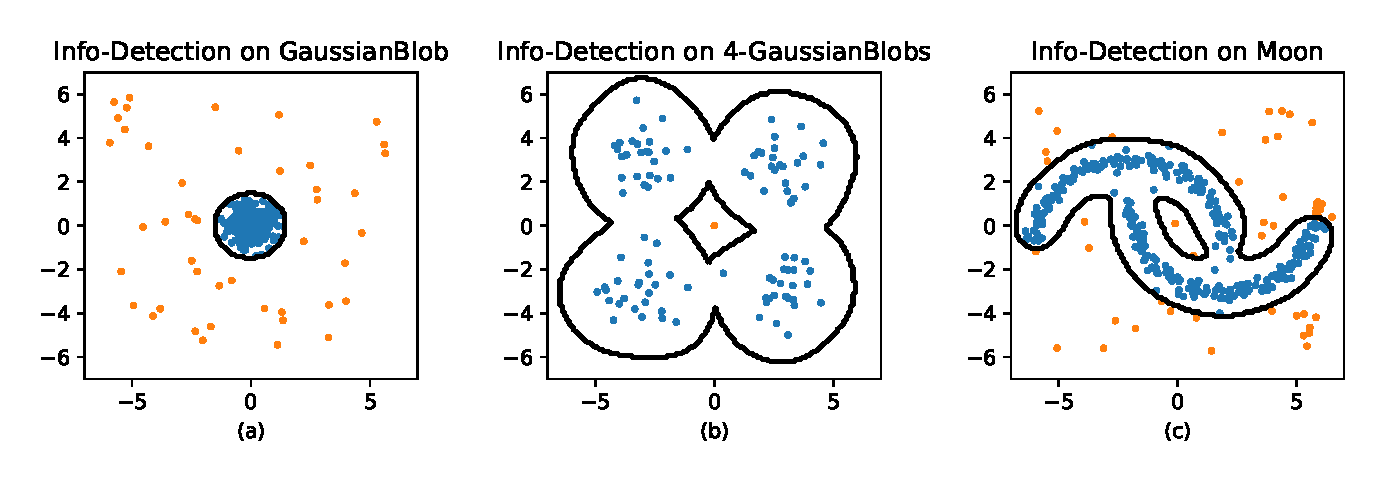
\includegraphics[width=\textwidth]{pic/outlier_boundary_illustration.eps}
	\caption{Detection boundary lines of different methods on different artificial dataset}	\label{fig:boundary}
\end{figure}

For outlier detection tasks, we also compare GBIC with other commonly used techniques on three datasets: Gaussian-blob, Moon and UCI Lymphography. The first two dataset are artificially generated as mentioned above. The third one is of 148 samples with 6 outliers. The other methods include local outlier factor \citep{Breunig}, isolation forest \citep{if}, elliptic envelope \citep{rousseeuw1999fast} and one class SVM \citep{svm}. We use TPR and TNR to measure the overall performance of the detection. The inlier is treated as positive sample. TPR measures the percentage of right detection in inlier set while TNR measures that in outlier set. It is difficult for a method to achieve high score on both two metrics. We manage to maximize TNR while controlling TPR $\geq 90\%$ for each method. The hyper parameters and metric are tuned for each method and the best result of TNR is shown in Table \ref{tab:odm}. We can see that GBIC is competitive with local outlier factor and outperforms other methods on these datasets.

\begin{table}
\centering
\begin{tabular}{cccc}
\hline
       TPR/TNR        &  GaussianBlob   &      Moon       &  Lymphography  \\
\hline
    Info-Detection    & 100\%/100\% &  96.7\%/82.2\%  & 97.9\%/100\% \\
 local outlier factor & 100\%/100\% & 100\%/100\% & 98.6\%/83.3\%  \\
   isolation forest   & 100\%/100\% &  96.7\%/77.8\%  & 99.3\%/100\% \\
  elliptic envelope   & 100\%/100\% &  91.3\%/42.2\%  & 93.7\%/100\% \\
    one class SVM     &  98.8\%/91.1\%  &  93.0\%/55.6\%  & 93.0\%/66.7\%  \\
\hline
\end{tabular}
\caption{Comparison of different outlier detection methods}\label{tab:odm}
\end{table}

The method presented in this section is an extension of Info-Detection \citep{zhao2019info}, in which the inliers are assumed to be of one class. Therefore it can handle more general cases and
jointly do outliers and clustering tasks.

\section{Conclusion}\label{sec:conc}
In this paper, we consider a special model of info-clustering: graph-based info-clustering (GBIC). We also propose an efficient algorithm to compute the principal sequence of partition for a graph, which is used to deduce the hierarchical structures of GBIC. Empirical study shows that GBIC can be applied to many fields and it performs well on a wide range of datasets. Our method is especially suitable if the hierarchical tree structure of data is preferred and to remove outliers from multiple-class datasets.
%\begin{acknowledgements}
%If you'd like to thank anyone, place your comments here
%and remove the percent signs.
%\end{acknowledgements}


% Authors must disclose all relationships or interests that 
% could have direct or potential influence or impart bias on 
% the work: 
%
\section*{Conflict of interest}
%
The authors declare that they have no conflict of interest.


% BibTeX users please use one of
\bibliographystyle{spbasic}      % basic style, author-year citations
%\bibliographystyle{spmpsci}      % mathematics and physical sciences
%\bibliographystyle{spphys}       % APS-like style for physics
\bibliography{exportlist.bib}   % name your BibTeX data base

% Non-BibTeX users please use
%\begin{thebibliography}{}
%
% and use \bibitem to create references. Consult the Instructions
% for authors for reference list style.
%
%\bibitem{RefJ}
% Format for Journal Reference
%Author, Article title, Journal, Volume, page numbers (year)
% Format for books
%\bibitem{RefB}
%Author, Book title, page numbers. Publisher, place (year)
% etc
%\end{thebibliography}
\appendix
\section{Proofs}
\subsection{Proof of Theorem \ref{thm:DPX}}
We need the following Lemma to prove Theorem \ref{thm:DPX}:
\begin{lemma}\label{lem:xyz}
	If $(X,Y)$ is weakly dependent with $Z$, then $X$ is weakly dependent with $Z$.
\end{lemma}
\begin{proof}
	From the definition of weak dependence for two random variables, we have
	\begin{equation}
	P_{X,Y|Z=z}(x,y) = P_{X,Y}(x,y)(1+\epsilon \frac{\phi_z(x,y)}{\sqrt{P_{X,Y}(x,y)}}), z \in \mathcal{Z}
	\end{equation}
	Summing the above equation over $y\in \mathcal{Y}$ we have
	\begin{equation}
	P_{X|Z=z}(x) = P_X(x)(1+\epsilon\frac{\tilde{\phi}_z(x)}{\sqrt{P_X(x)}}),
	\textrm{ where } \tilde{\phi}_z(x) = \frac{\sum_{y\in Y} \sqrt{P_{X,Y}(x,y) }\phi_z(x,y)}{\sqrt{P_X(x)}}
	\end{equation}
	which implies $X$ is weakly dependent with $Z$.
\end{proof}
\begin{proof}[Proof of Theorem \ref{thm:DPX}]
From the definition of weak dependence for more than 2 random variables, we can find a discrete distribution $U$ over $\{1, 2,\dots, K\}$, such that $Z_1, \dots, Z_n$ are independent conditioned on $U$. Since $(Z_1, \dots, Z_n)$ is weakly dependent with $U$, from Lemma \ref{lem:xyz}, it follows that $Z_i$ is weakly dependent with $U$.  That is, 
\begin{equation}\label{XUk}
P_{Z_i | U=k}(z) = P_{Z_i} (z)( 1 + \epsilon {\phi^{(k,i)}(z) \over \sqrt{P_{Z_i}(z)}} )
\end{equation}
We then have
\begin{align}
P_{Z_i, Z_j | U = k}(z_i, z_j)
=& P_{Z_i | U=k}(z_i)
P_{Z_j | U=k}(z_j) \notag \\
=& P_{Z_i}(z_i)P_{Z_j}(z_j)
(1 + \epsilon(\frac{\phi^{(k,i)}(z_i)}{\sqrt{P_{Z_i}(z_i)}}
+ \frac{\phi^{(k,j)}(z_j)}{\sqrt{P_{Z_j}(z_j)}}) +
\epsilon^2\frac{\phi^{(k,i)}(z_i)
	\phi^{(k,j)}(z_j)}{\sqrt{P_{Z_i}(z_i)P_{Z_j}(z_j)}})\label{eq:XiXj}
\end{align}
Since 
\begin{align*}
P_{Z_i}(z) &= \sum_{k=1}^{K} P_{Z_i | U=k}(z) P_U(u_k) \\
& =  \sum_{k=1}^{K}P_U(u_k)P_{Z_i} (z)( 1 + \epsilon {\phi^{(k,i)}(z) \over \sqrt{P_{Z_i}(z)}} ) \textrm{ from } \eqref{XUk}\\
\Rightarrow & \sum_{k=1}^{K} P_U(u_k){\phi^{(k, i)}(z) \over \sqrt{P_{Z_i}(z)}} =0,\forall i, z\in \mathcal{Z}
\end{align*}
From \eqref{eq:XiXj} we have
\begin{equation}\label{eq:PXiXj}
P_{Z_i, Z_j}(z_i, z_j) = P_{Z_i}(z_i)
P_{Z_j}(z_j) (1+\epsilon^2 \sum_{k=1}^K P_U(u_k)
\frac{\phi^{(k,i)}(z_i)
	\phi^{(k,j)}(z_j)}{\sqrt{P_{Z_i}(z_i)P_{Z_j}(z_j)}})
)
\end{equation}
For more than 2 random variables:
\begin{align*}
P_{Z_1,\dots,Z_n}(z_1,\dots,z_n)  &= \sum_{k=1}^{K} P_{Z_1,\dots,Z_n | U=k}(z_1,\dots,z_n) P_U(u_k) \\
&=  \sum_{k=1}^{K}P_U(u_k) \prod_{i=1}^n P_{Z_i|U=k}(z_i)\\
&= \sum_{k=1}^{K} P_U(u_k)\prod_{i=1}^n \left(P_{Z_i} (z_i)( 1 + \epsilon {\phi^{(k,i)}(z_i ) \over \sqrt{P_{Z_i}(z_i)}} )\right)\\
&=  \sum_{k=1}^{K}P_U(u_k) (\prod_{i=1}^n  P_{Z_i} (z_i))
\left( 1 + \epsilon\sum_{i=1}^n {\phi^{(k,i)}(z_i) \over \sqrt{P_{Z_i}(z_i)}} + \epsilon^2\sum_{i\neq j}{\phi^{(k,i)}(z_i)\phi^{(k,j)}(z_j)\over \sqrt{P_{Z_i}(z_i)P_{Z_j}(z_j)} }\right)+o(\epsilon^2) \\
&= (\prod_{i=1}^n  P_{Z_i} (z_i))
(1+\epsilon\sum_{i=1}^n \sum_{k=1}^{K} P_U(u_k){\phi^{(k,i)}(z_i) \over \sqrt{P_{Z_i}(z_i)}} \\
&+\epsilon^2 \sum_{k=1}^{K} P_U(u_k)\sum_{i\neq j}{\phi^{(k,i)}(z_i)\phi^{(k,j)}(z_j)\over \sqrt{P_{Z_i}(z_i)P_{Z_j}(z_j)} } ) + o(\epsilon^2)\\
&= (\prod_{i=1}^n  P_{Z_i} (z_i))
\left(1 +\epsilon^2\sum_{i\neq j} \sum_{k=1}^{K}P_U(u_k){\phi^{(k,i)}(z_i)\phi^{(k,j)}(z_j)\over \sqrt{P_{Z_i}(z_i)P_{Z_j}(z_j)} }\right) + o(\epsilon^2)
\end{align*}
From \eqref{eq:PXiXj},
let $B_{ij}(z_i, z_j)={P_{Z_i, Z_j}(z_i,z_j) - P_{Z_i}(z_i)P_{Z_j}(z_j) \over \sqrt{P_{Z_i}(z_i)P_{Z_j}(z_j)}} $, then we have:
\begin{align}
\epsilon^2\sum_{k=1}^{K}P_U(u_k)
{\phi^{k,i}(z_i)\phi^{k,j}(z_j)\over \sqrt{P_{Z_i}(z_i)P_{Z_j}(z_j)} } & = {P_{Z_i, Z_j}(z_i, z_j) - P_{Z_i}(z_i)P_{Z_j}(z_j) \over P_{Z_i}(z_i)P_{Z_j}(z_j)} \notag\\
& = {B_{ij}(z_i, z_j) \over \sqrt{P_{Z_i}(z_i)P_{Z_j}(z_j)} } \label{eq:Bsecond}
\end{align}
Therefore, we have 
\begin{equation}\label{eq:sep}
P_{Z_1,\dots,Z_n}(z_1,\dots,z_n) =  (\prod_{i=1}^n  P_{Z_i} (z_i))\left ( 1 + \sum_{i\neq j}{B_{ij}(z_i, z_j) \over \sqrt{P_{Z_i}(z_i)P_{Z_j}(z_j)} }\right) +o(\epsilon^2)
\end{equation}
Then $P_{Z_1,\dots, Z_n}$ is in the neighborhood of $P_{Z_1}\dots P_{Z_n}$ with $$\phi(z_1,\dots, z_n)=
\sqrt{P_{Z_1}(z_1)\dots P_{Z_n}(z_n)}\left(\sum_{i\neq j}{B_{ij}(z_i, z_j) \over \sqrt{P_{Z_i}(z_i)P_{Z_j}(z_j)} }\right)+o(\epsilon^2)$$

Using Equation \eqref{eq:approx:ig} from information geometry:
\begin{align*}
D(P_{Z_1,\dots, Z_n}|| P_{Z_1}\dots P_{Z_n}) & ={1 \over 2} \sum_{z_1,\dots,z_n}\phi^2(z_1,\dots, z_n) \\
& = {1\over 2}\sum_{z_1,\dots,z_n} (\prod_{i=1}^n  P_{Z_i} (z_i)) \left(\sum_{i\neq j}{B_{ij}(z_i, z_j) \over \sqrt{P_{Z_i}(z_i)P_{Z_j}(z_j)} }\right)^2 +o(\epsilon^2) 
\end{align*}
From the definition of $B_{ij}$, the above is the summation over $\norm{B_{ij}}^2_F$(the coupling term is zero).
Therefore we get the second order approximation for the total partition:
\begin{equation}
D(P_{Z_1,\dots, Z_n}|| P_{Z_1}\dots P_{Z_n}) =   {1 \over 2} \sum_{i\neq j} \norm{B_{ij}}^2_F + o(\epsilon^2)
\end{equation}
For an arbitrary partition $\P$, using Equation \eqref{eq:sep} for each $C\in \P$, we have
\begin{equation}
P_{Z_C}(z_C) = \prod_{i\in C} P_{Z_i}(z_i)(1 + \epsilon^2 \sum_{i\neq j,i,j\in C} \frac{B_{ij}(z_i, z_j)}{\sqrt{P_{Z_i}(z_i)P_{Z_j}(z_j)}}) + o(\epsilon^2)
\end{equation}
Multiplying these equations and notice $\frac{\tilde{B}_{ij}(z_i, z_j)}{\sqrt{P_{Z_i}(z_i)P_{Z_j}(z_j)}}=O(\epsilon^2)$ from
Equation \eqref{eq:Bsecond} we have:
\begin{equation}
\prod_{C\in \P}P_{Z_C}(z_C) = \prod_{i=1}^n P_{Z_i}(z_i)(1+\epsilon^2 \sum_{C\in\P}\sum_{i\neq j,i,j\in C}\frac{B_{ij}(z_i, z_j)}{\sqrt{P_{Z_i}(z_i)P_{Z_j}(z_j)}}) + o(\epsilon^2)
\end{equation}
Then $\prod_{C\in \P}P_{Z_C}$ is in the neighborhood of $P_{Z_1}\dots P_{Z_n}$ with $$\phi_{\P}(z_1,\dots, z_n)=
\sqrt{P_{Z_1}(z_1)\dots P_{Z_n}(z_n)}\left(\sum_{C\in\P}\sum_{i\neq j,i,j\in C}\frac{B_{ij}(z_i, z_j)}{\sqrt{P_{Z_i}(z_i)P_{Z_j}(z_j)}}\right)+o(\epsilon^2)$$
Applying Equation  \eqref{eq:approx:ig} we have:
\begin{align*}
D(P_{Z_1,\dots, Z_n}|| \prod_{C\in \P}P_{Z_C}) & ={1 \over 2} \sum_{z_1,\dots,z_n}(\phi(z_1,\dots, z_n)-\phi_{\P}(z_1, \dots, z_n))^2 \\
& = {1\over 2}\sum_{z_1,\dots,z_n} (\prod_{i=1}^n  P_{Z_i} (z_i)) \left(\sum_{\substack{(i,j) \not\in C\\ C\in \P}} {B_{ij}(z_i, z_j) \over \sqrt{P_{Z_i}(z_i)P_{Z_j}(z_j)} }\right)^2 +o(\epsilon^2) \\
& = \frac{1}{2} \sum_{\substack{(i,j) \not\in C\\ C\in \P}} \norm{B_{ij}}_F^2 + o(\epsilon^2)
\end{align*}
\end{proof}
\subsection{Proof of Proposition \ref{prop:triangle}}
\begin{lemma}\label{lem:trival}
	The partition to minimize equation \eqref{eq:ms} is $\P_k = \{\{1\},\{2\},\dots,\{\abs{V}\}\}$ if and only if equation \eqref{eq:GF2} holds.
	\begin{equation}\label{eq:GF2}
	\frac{f[\P]}{\abs{\P}-1} \geq \frac{f[\P_k]}{\abs{V}-1} \textrm{ for any } \P \in \Pi'
	\end{equation}
\end{lemma}
\begin{proof}
	The partition is trivial if and only if Line \ref{line:11} is hit in Algorithm \ref{alg:psp} for the first invocation if \texttt{Split}.
	Since $Q=\{V\}$, $f[Q]=0$. Let $\P_k = \{\{i\} | i \in V\}$, then $ f[P] = f[\P_k]$. We then have$(\gamma', h')=(\lambda_{+}, -\lambda_{+})$ where $\lambda_{+} = \frac{f[\P_k]}{\abs{V}-1}$. Since $\frac{f[\P]}{\abs{\P}-1} \geq \lambda_{+} \iff f[\P] - \abs{\P}\lambda_{+} \geq - \lambda_{+} \iff \tilde{h}(\lambda_{+}) = - \lambda_{+}$. Then the conclusion follows.
\end{proof}

\begin{proof}[Proof of Proposition \ref{prop:triangle}]
By Lemma \ref{lem:trival}, we only need to show
\begin{equation}\label{eq:GF}
f[\P] \geq \frac{\abs{\P}-1}{\abs{V}-1} \sum_{(i,j) \in E} w_{ij}
\end{equation}
holds for any $\P \in \Pi$. We prove Equation \ref{eq:GF} in a deductive way.

Let $n=\abs{V}$. For $\abs{\P}=n$, the equality of equation \ref{eq:GF} holds. 

Suppose equation \eqref{eq:GF} holds for any $\abs{\P} \geq k+1(k\geq 2)$, and for $\P=\{C_1, \dots, C_k\}$, with $\abs{C_1} \geq \abs{C_r}$ for $r=2,\dots, k$. Let $\abs{C_1}=n_1(\geq 2), \P_{C_1} = \{\{i\}| i \in C_1\}, \P'=\P_{C_1} \cup \P \backslash \{C_1\}$. Then we have $\abs{\P'} = k+n_1-1$. Using equation \eqref{eq:GF} for $\P'$ we have
\begin{align}\label{eq:PPrelation}
f[\P'] & \geq \frac{k+n_1 -2}{n-1}\sum_{(i,j) \in E} w_{ij} \\
f[\P] & =f[P'] - \sum_{(i,j) \in E(C_1)} w_{ij}
\end{align}
Applying triangle inequality $w_{ij} \leq w_{ik} + w_{jk}$ for given $k\not\in C_1$ and sum it over all $i, j \in C_1, i\neq j$, we have
$$
\sum_{(i,j) \in E(C_1)} w_{ij} \leq \sum_{(i,j) \in E(C_1)} (w_{ik} + w_{jk}) = (n_1-1)\sum_{i\in C_1} w_{ik}
$$
Summation over $k \not\in C_1$ we have 
$$
(n - n_1) \sum_{(i,j) \in E(C_1)} w_{ij} \leq (n_1 - 1) \sum_{i \in C_1, k \not\in C_1} w_{ik}
$$
Also
\begin{align*}
\sum_{(i,j) \in E} w_{ij}  & \geq \sum_{(i,j) \in E(C_1)} w_{ij} + \sum_{i\in C_1, k\not\in C_1} w_{ik} \\
(n_1 - 1)\sum_{(i,j) \in E} w_{ij}  & \geq (n_1 -1 )\sum_{(i,j) \in E(C_1)} w_{ij} + (n_1-1)\sum_{i\in C_1, k\not\in C_1} w_{ik} \\
& \geq (n_1 -1 )\sum_{(i,j) \in E(C_1)} w_{ij} + (n - n_1) \sum_{(i,j) \in E(C_1)} w_{ij}\\
& = (n-1) \sum_{(i,j) \in E(C_1)} w_{ij}
\end{align*}
We then have $\sum_{(i,j) \in E(C_1)} w_{ij} \leq \frac{n_1-1}{n-1}\sum_{(i,j) \in E} w_{ij}$. From equation \eqref{eq:PPrelation} we have 
$f[\P] \geq \frac{k-1}{n-1}\sum_{(i,j) \in E} w_{ij}$. That is, the result holds for $\abs{\P}=k$.
\end{proof}


\subsection{Proof of Proposition \ref{prop:reweight}}
We need the following lemmas to prove Proposition \ref{prop:reweight}.
\begin{lemma}[Corollary 5.1 in \cite{secretKey}]\label{lemma:laminarity}
	\begin{equation}\label{eq:P}
	I(Z_{C_1 \cup C_2}) \geq \min\{ I(Z_{C_1}), I(Z_{C_2})\}, \textrm{ for } C_1\cap C_2 \neq \emptyset
	\end{equation}
\end{lemma}
\begin{lemma}\label{lemma:sub}
	If node set $S_1 \cap S_2 \neq \emptyset, S_1 \not\subseteq S_2$ and $I(Z_{S_1}) \geq I(Z_{S_2})$, then $S_2$ is not a cluster of $G$.
\end{lemma}
\begin{proof}
	From Lemma \ref{lemma:laminarity},
	$I(Z_{S_1\cup S_2}) \geq \min\{I(Z_{S_1}), I(Z_{S_2})\} = I(Z_{S_2})$. Since $S_1 \cup S_2 \supsetneq S_2$, from the definition of info-clustering, $S_2$ cannot be a cluster of $G$.
\end{proof}
\begin{corollary}\label{cor:complete}
	For a complete graph $G(V,E)$ with equal weight $w$ on each edge, we have $I(Z_{V})=\frac{nw}{2}$ where $n=\abs{V}$. And $I(Z_S) < I(Z_V)$ for any subset $S\subsetneq V$.
\end{corollary}
\begin{proof}
	From Proposition \ref{prop:triangle}, $I(Z_{V})$ is achieved by $\P=\{\{1\},\dots,\{n\} \}$ and $I(Z_V) = I_{\P}(Z_V) = \frac{n(n-1)w/2}{n-1} = \frac{nw}{2} $. From Equation \eqref{eq:largest_threshold}, $I(Z_V) = \max_{S\subset V} I(Z_S)$, therefore $I(Z_S) \leq I(Z_V)$. If $I(Z_S) = I(Z_V)$ for some $S\subsetneq V$, consider $\P_S=\{i | i \in S\}$, then $I(Z_S) = I_{\P_S}(Z_S) = \frac{\abs{S}w}{2} < I(Z_V)$, a contradiction. Therefore, $I(Z_S) < I(Z_V)$ holds for any subset $S\subsetneq V$.
\end{proof}
\begin{proof}[Proof of Proposition \ref{prop:reweight}]
If $m < \frac{nr}{2}$, we will show that if $U \neq S_1$ and $U \neq S_2$, $U$ cannot be a cluster of $G$.
	
For any $U \in S_1 \cup S_2 $ and $\abs{U} \leq n$, If $U \in S_1$ or $U \in S_2$, then by Corollary \ref{cor:complete}, $I(Z_U) < I(Z_{S_1})$.
If $U \cap S_1 \neq \emptyset$ or $U \cap S_2 \neq \emptyset$ holds, $I(Z_{S_1})= I(Z_{S_2}) = \frac{nr}{2} > m \geq I_{\{U \cap S_1, U \cap S_2\}} \geq I(Z_U) \Rightarrow U$ is not a cluster of $G$ from Lemma \ref{lemma:laminarity}.

For $\abs{U} > n$ but $U \neq V = S_1 \cup S_2$. Suppose $S_2 \subset U$. Let $\P' = \{\{i\}| i\in U\}$, $I(Z_U) \leq I_{\P'}(Z_U) = \frac{\frac{rn(n-1)}{2} + m + \frac{rk(k-1)}{2}}{n+k-1}$ where $m_1 \leq nk$ and $k=\abs{U} - n < n$. 
We compare it to $I(Z_{S_1}) = \frac{nr}{2}$ and we can show that $I(Z_{S_1}) - I_{\P'}(Z_U) \geq \frac{nrk-2m-rk(k-1)}{2(n+k-1)}$. 

Using $m<\frac{nr}{2}$, $I(Z_{S_1}) - I_{\P'}(Z_U) > \frac{r(n-k)(k-1)}{2(n+k-1)} \geq 0$. Then $I(Z_{S_1})>I(Z_U)$, $U$ is not a cluster by Lemma \ref{lemma:sub}. In either case, $U$ is not a cluster of $G$ for $1<\abs{U}<2n, U \neq S_1, U\neq S_2$. Based on this conclusion, by simply comparing $I_{\P}(Z_V) = \frac{m+rn(n-1)}{2n-1}$ with
$ I_{\{S_1, S_2\}}=m$ we can conclude that $I(Z_V) = I_{\{S_1, S_2\}}$ when $ m < \frac{nr}{2}$. Therefore, $S_1$ and $S_2$ can be simultaneously discovered by GBIC.

If $m \geq \frac{nr}{2}$, we have $I_{\P}(Z_V) = \frac{m+rn(n-1)}{2n-1} \leq m = I_{\{S_1, S_2\}}(Z_V)$.
Suppose $I(Z_V) = I_{\P^*}(Z_V)$.
If $S\in \P^*$ and $S\subseteq S_1$. From Lemma \ref{lemma:sub} we must have $S=S_1$. Then $\P^*=\{S_1, S_2\}$, which contradicts with
$I_{\P}(Z_V)  \leq  I_{\{S_1, S_2\}}(Z_V)$ since $\P$ is finer than $\{S_1, S_2\}$. The same can be said if $S\in \P^*$ and $S\subseteq S_2$.
Therefore, neither $S_1$ nor $S_2$ can be discovered.

\end{proof}
\subsection{Proof of Proposition \ref{prop:main}}
\begin{proof}[Proof of Proposition \ref{prop:main}]
	In this proof, we make some notation convention.
	$w(C) = \displaystyle\sum_{(i,j) \in E(C)} w_{ij},$
	$w(A, C) = \displaystyle\sum_{\substack{i \in A, j \in C \\ (i,j) \in E(V')}} (w_{ij}+w_{ji})$ and
	$\P_C = \{\{i \}| i \in C \}$. Suppose $\gamma_N = I(Z_B)$, from equation \eqref{eq:largest_threshold}, we can get $\gamma_N =\frac{f[\P_B]} {\abs{B} -1}$.
	Since $V' = B \cup \{i'\}$
	$f[\P_{V'}] = f[\P_B] + \sum_{i \in B}w_{ii'}$.
	
	If $ \sum_{i \in B} w_{ij} > \gamma_N$ we can get
	$$
	\gamma'_N \geq I_{\P_{V'}}(Z_{V'}) = \frac{(\abs{B}-1)\gamma_N + \sum_{i \in B}w_{ii'}}{\abs{B}} > \gamma_N
	$$
	
	On the other hand, suppose $\gamma'_N = I(Z_K) > \gamma_N$. Then $K$ must contain $i'$. If $K=V'$ then the conclusion holds. Otherwise, Suppose $K = \{i'\} \cup B', B=B'\cup J, J\neq \emptyset$. We can write 
	\begin{equation}\label{eq:gammaNF}
	\gamma_N = \frac{w(J,B') + w(J) + w(B')}{ \abs{B'} + \abs{J} - 1 }
	\end{equation}
	Since $I(Z_K) = I_{\P_K}(Z_K)$ is maximal, we have $I_{\P_K}(Z_K) > I_{\P_{V'}}(Z_{V'})$ and $I_{\P_K}(Z_K) \geq I_{\P_{B'}}(Z_{B'})$.
	\begin{align*}
	\frac{w(\{i'\}, B') + w(B')}{\abs{B'}} >& \frac{w(B') + w(J, B') + w(J) + w(\{i'\}, B') + w(\{i'\}, J)}{\abs{B'} + \abs{J}}  \\
	\frac{w(\{i'\}, B') + w(B')}{\abs{B'}} \geq & \frac{w(B')}{\abs{B'} - 1}
	\end{align*}
	we can get 
	\begin{align}
	\abs{J} (w(\{i'\}, B') + w(B')) > & \abs{B'} (w(J, B') + w(J) + w(\{i'\}, J)) \label{eq:target}
	\\
	(\abs{B'} - 1)  w(\{i'\}, B') \geq & w(B') \label{eq:convert}
	\end{align}
	Taking equation \eqref{eq:convert} in \eqref{eq:target}, we can get
	\begin{equation}\label{eq:summation}
	\abs{J} w(\{i'\}, B') > w(J, B') + w(J) + w(\{i'\}, J)
	\end{equation}	
	Combined with \eqref{eq:gammaNF}, adding equation \eqref{eq:convert} and \eqref{eq:summation} we can get
	$w(\{i'\}, B') > \gamma_N$. Then $\sum_{j \in B}w_{ii'} > \gamma_N $ follows.
\end{proof}
\subsection{Proof of Proposition \ref{prop:alg_complexity}}
\begin{proof}[Proof of Proposition \ref{prop:alg_complexity}]
Let $\mu_i = \frac{n_i}{n} \leq \frac{1}{2}$. We proceed by induction to show $T(n) = O(n^4)$. More specifically, $T(n) \leq q C n^4$ where $ q = \frac{16}{5}$. $T(3)$ is a constant and $T(m) \leq q C m^4$ holds for $m=3$. Suppose
	$T(m) \leq qC m^4$ holds for all $m \leq n-1$. Then for $T(n)$
	we first show that 
	\begin{equation}\label{eq:outerI}
	\sum_{i=1}^k T(n_i) \leq 10 T(\frac{n}{2})
	\end{equation}
	Since $\sum_{i=1}^k T(n_i) \leq qC n^4\sum_{i=1}^k u_i^4$ and $10 T(\frac{n}{2}) \geq 10Cn^4 (\frac{1}{2})^4$ from equation \eqref{eq:Tn}
	\begin{equation}\label{eq:innerI}
       q\sum_{i=1}^k u_i^4 \leq 10 (\frac{1}{2})^4 
	\end{equation}
	We have \eqref{eq:innerI} $\Rightarrow$ \eqref{eq:outerI}. The constraint is that $u_1\leq u_2 \leq \dots \leq u_k \leq \frac{1}{2}$ and $\sum_{i=1}^k u_i = 1$. Therefore we have $u_1 \leq \frac{1}{k}, u_2 \leq \frac{1}{k-1}, \dots, u_{k-1} \leq \frac{1}{2}$.
	\begin{equation}\label{eq:outerOne}
	 q[2(\frac{1}{2})^4 + \sum_{i=3}^k (\frac{1}{i})^4] \leq 10 (\frac{1}{2})^4
	\end{equation}
	We have \eqref{eq:outerOne} $\Rightarrow$ \eqref{eq:innerI}. And \eqref{eq:outerOne} is equivalent to
	$\sum_{i=3}^k (\frac{1}{i})^4 \leq \frac{9}{8}(\frac{1}{2})^4$
	\begin{align*}
		\sum_{i=3}^k (\frac{1}{i})^4 & < \frac{1}{9}\sum_{i=3}^k (\frac{1}{i})^2 \\
		& < \frac{1}{9}\sum_{i=3}^k (\frac{1}{(i-1)i}) \\
		& < \frac{1}{18} < \frac{9}{8}(\frac{1}{2})^4
	\end{align*}
	Therefore, \eqref{eq:outerI} holds and from \eqref{eq:Tn} and $T(k) \leq T(\frac{n}{2})$ we have 
	\begin{align}
		T(n)  & \leq Cn^4 + 11T(\frac{n}{2}) \\
		& \leq C n^4 + 11 q C (\frac{n}{2})^4 = \frac{16}{5} C n^4
	\end{align}
\end{proof}	
\end{document}
% end of file template.tex

